\documentclass[11pt,a4paper]{report}

\usepackage[utf8]{inputenc}
\usepackage[margin=1in]{geometry}
\usepackage{amsmath,amssymb,amsfonts,amsthm}
\usepackage{graphicx}
\usepackage{booktabs}
\usepackage{multirow}
\usepackage{array}
\usepackage{hyperref}
\usepackage{xcolor}
\usepackage{algorithm}
\usepackage{algorithmic}
\usepackage{fancyhdr}
\usepackage{caption}
\usepackage{subcaption}
\usepackage{cite}
\usepackage{enumitem}

\hypersetup{
    colorlinks=true,
    linkcolor=blue!70!black,
    citecolor=green!50!black,
    urlcolor=blue!80!black
}

\graphicspath{{visualization/figures/}}

\pagestyle{fancy}
\fancyhf{}
\rhead{\small\textit{Time-Series Counterfactual Explanations}}
\lhead{\small\textit{Soft-DTW to DTW-Guided Deformation}}
\cfoot{\thepage}

\begin{document}

% ==============================================================================
% TITLE PAGE
% ==============================================================================
\begin{titlepage}
    \centering
    \vspace*{1.5cm}
    
    {\Huge \bfseries Plausibility, Proximity, and Computational Efficiency in Time-Series Counterfactual Explanations\par}
    \vspace{0.8cm}
    {\LARGE From Soft-DTW Optimization to DTW-Guided Constrained Deformation\par}
    
    \vspace{2.0cm}
    
    {\Large \textbf{Comprehensive Project Report and Monograph}}\\[0.5cm]
    {\large Repository: \texttt{soft\_dtw\_cfe}}\\[0.3cm]
    {\large Reference Paper: Kostrzewa, Galus, and Zięba (arXiv:2603.08349, 2026)}\par
    
    \vfill
    
    \begin{minipage}{0.8\textwidth}
        \centering
        \textbf{Abstract Overview:}\\
        \textit{An exhaustive technical investigation into the multi-objective trade-offs of time-series counterfactual recourse. Evaluates Soft-DTW gradient optimization, latent-space autoencoders, heuristic subsequence replacement, and introduces a novel DTW-Guided Constrained Deformation architecture via CMA-ES across 8 UCR/UEA benchmark datasets.}
    \end{minipage}
    
    \vspace{1.5cm}
    {\large \today}\par
\end{titlepage}

% ==============================================================================
% FRONT MATTER
% ==============================================================================
\pagenumbering{roman}

\tableofcontents
\newpage
\listoffigures
\newpage
\listoftables
\newpage

\pagenumbering{arabic}

% ==============================================================================
% 1. ABSTRACT
% ==============================================================================
\chapter{Abstract}
Counterfactual explanations (CFEs) offer an intuitive and actionable paradigm for post-hoc Explainable Artificial Intelligence (XAI) by identifying minimal, physically plausible perturbations that reverse a predictive model's decision. In Time-Series Classification (TSC), classical counterfactual generation algorithms relying on pointwise Euclidean ($L_1, L_2$) metrics systematically produce unphysical artifacts—such as high-frequency oscillatory noise, unnatural amplitude spikes, and phase-delayed step discontinuities. These artifacts stem directly from the rigid point-to-point temporal alignment assumption inherent in Euclidean formulations. 

Recently, Kostrzewa, Galus, and Zięba (arXiv:2603.08349, 2026) introduced \textbf{Soft-DTW CFE}, which incorporates differentiable soft dynamic time warping directly into the counterfactual loss function to encourage morphological alignment with target-class prototypes. While Soft-DTW substantially improves morphological plausibility and in-distribution nominality, incorporating the dynamic programming trellis directly into the iterative optimization loop induces a severe computational bottleneck: an $\mathcal{O}(I \cdot K \cdot T^2)$ time complexity, where $I$ represents optimization iterations, $K$ the number of target reference prototypes, and $T$ sequence length. On long multivariate sequences such as Cricket ($T=1197, d=6$), generation requires over 91 seconds per sample, severely restricting its practical deployment in clinical telemetry or industrial cyber-physical monitoring.

To resolve this trade-off, this report provides a thorough reproduction, comparative benchmarking, and algorithmic extension of time-series counterfactual explanations. We benchmark Soft-DTW CFE against established state-of-the-art baselines (Glacier and M-CELS) across eight diverse UCR/UEA benchmark datasets. Furthermore, we develop and evaluate a novel paradigm: \textbf{DTW-Guided Constrained Deformation via Covariance Matrix Adaptation Evolution Strategy (CMA-ES)}. By extracting the elastic DTW temporal alignment once as a continuous geometric prior into an 8-dimensional Radial Basis Function (RBF) velocity and amplitude space, our proposed method decouples the quadratic cost from the inner search loop, collapsing optimization complexity to $\mathcal{O}(K \cdot T^2 + I_{\text{CMA}} \cdot d \cdot T)$.

Our empirical results demonstrate that on long multivariate sequences (Cricket), DTW-CFE achieves a \textbf{44.4$\times$ runtime speedup} (2.05 s/sample vs. 91.12 s/sample for Soft-DTW), while boosting target-class validity from 50.0\% to 100.0\%. On univariate datasets with moderate length, Soft-DTW CFE maintains superior DTW plausibility and high Isolation Forest nominal scores (up to 1.000). We conclude with a comprehensive comparative analysis, failure mode taxonomy, and an explicit visual placement guide linking empirical figures to analytical findings.

% ==============================================================================
% 2. INTRODUCTION
% ==============================================================================
\chapter{Introduction}

\section{The Rise of Deep Learning in Time-Series Classification (TSC)}
Time-series data is ubiquitous across modern industrial, scientific, and medical systems. From electrocardiogram (ECG) rhythm monitoring and seismological tremor detection to smart grid electricity load forecasting and gestural motion capture, temporal sequences encode critical physical processes. Over the past decade, deep neural networks—especially One-Dimensional Convolutional Neural Networks (1D-CNNs), Residual Networks (ResNets), and Temporal Convolutional Networks (TCNs)—have achieved state-of-the-art classification accuracy on the benchmark UCR and UEA archives \cite{ismail2019deep, dau2019ucr, bagnall2017uea}. 

Despite their impressive accuracy, deep neural architectures operate as opaque ``black-box'' non-linear functions. In safety-critical sectors, such as clinical cardiology or automated power grid dispatch, deploying uninterpretable models presents grave operational and ethical hazards. Human experts cannot blindly trust predictions without understanding the underlying reasoning, necessitating post-hoc Explainable Artificial Intelligence (XAI) methodologies \cite{guidotti2018survey}.

\section{Explainable AI (XAI) and the Imperative for Counterfactuals}
Early XAI techniques for time series primarily adapted feature attribution mechanisms, including Saliency Maps, Grad-CAM, and Temporal SHAP. These methods highlight specific time intervals or frequency bands that contributed most significantly to a classification decision. However, feature attribution suffers from inherent limitations:
\begin{enumerate}[label=(\roman*)]
    \item \textbf{Lack of Actionability}: Highlighting that an abnormal ECG spike caused an arrhythmia diagnosis does not inform clinicians what morphological changes would revert the classification to normal sinus rhythm.
    \item \textbf{Susceptibility to Confirmation Bias}: Saliency heatmaps frequently highlight correlated background noise rather than causal features.
    \item \textbf{Inability to Test Hypotheses}: Feature attribution does not answer the question: \textit{``What is the smallest plausible change that would change the outcome?''}
\end{enumerate}

Counterfactual explanations (CFEs), formalized by Wachter et al. \cite{wachter2017counterfactual}, address these limitations directly. Given an input sequence $X$ classified as $y = f(X)$, a counterfactual explanation is a modified sequence $X'$ such that:
\begin{equation}
    f(X') = y_{\text{target}} \quad (y_{\text{target}} \neq y)
\end{equation}
while keeping the perturbation between $X$ and $X'$ minimal according to a suitable distance metric $\mathcal{D}(X, X')$. In medical diagnosis, this translates to identifying the minimum physiological change required to indicate patient recovery. In financial telemetry, it identifies the minimal transaction adjustment needed to clear a fraud alert.

\section{Fundamental Challenges in Time-Series Counterfactuals}
While counterfactual generation is well-established for tabular data and 2D images, time series introduce unique topological and physical constraints:
\begin{itemize}
    \item \textbf{Temporal Correlation and Ordering}: Adjacent time steps $x_t$ and $x_{t+1}$ are strongly coupled. Pointwise perturbations that disregard autocorrelation produce unphysical high-frequency jitter.
    \item \textbf{Phase Shifts and Non-Stationarity}: Two time series representing the identical underlying biological event may appear completely dissimilar under point-by-point comparisons due to temporal dilation, delay, or localized acceleration.
    \item \textbf{Data Manifold Plausibility}: Generated counterfactuals must not only flip the classifier's prediction, but also look like plausible physical signals. If $X'$ falls into an empty, off-manifold region of input space, the explanation is an adversarial artifact rather than a realistic recourse.
\end{itemize}

\section{Scope and Contributions of this Report}
This report provides an exhaustive investigation into the theory, implementation, and empirical performance of time-series counterfactual explanation methods. Specifically, we examine:
\begin{enumerate}
    \item \textbf{The Base Implementation \cite{kostrzewa2026towards}}: A complete implementation of the Soft-DTW Counterfactual Explanation framework, optimizing a four-component loss ($\mathcal{L}_{\text{prox}}, \mathcal{L}_{\text{sparse}}, \mathcal{L}_{\text{valid}}, \mathcal{L}_{\text{DTW}}$) via frozen-classifier gradient descent.
    \item \textbf{State-of-the-Art Baselines}: Comprehensive benchmarking against Glacier \cite{delaney2021instance} (an autoencoder latent-space perturbation method) and M-CELS \cite{wang2021large} (a heuristic multi-channel subsequence search method).
    \item \textbf{The Novel DTW-Guided Constrained Deformation Architecture}: Addressing the quadratic runtime bottleneck by extracting DTW alignment once as an empirical prior into an RBF velocity deformation space optimized via CMA-ES.
    \item \textbf{Empirical Benchmarking Across 8 Datasets}: Evaluating 20 test instances across three random seeds on 8 benchmark datasets spanning univariate, multivariate, short ($T=24$), and long ($T=1197$) temporal domains.
    \item \textbf{Systematic Visual Guidance}: Directing researchers and practitioners on where and how to integrate visualization figures, loss trajectories, and metric plots.
\end{enumerate}

% ==============================================================================
% 3. MOTIVATION
% ==============================================================================
\chapter{Motivation}

\section{The Failure of Pointwise Euclidean Distances in Temporal Dynamics}
The classical counterfactual objective minimizes an $L_1$ or $L_2$ norm between the original sample $X$ and the counterfactual $X'$:
\begin{equation}
    \mathcal{D}_{\text{Euc}}(X, X') = \frac{1}{d \cdot T} \sum_{c=1}^d \sum_{t=1}^T (X_{c,t}' - X_{c,t})^2
\end{equation}
While mathematically convenient and trivial to differentiate, Euclidean distance assumes strict point-to-point temporal alignment. Consider two cardiac pulses identical in shape, but with the second pulse delayed by $\Delta t = 10$ milliseconds. Under Euclidean distance, the squared error between the two pulses is nearly as large as comparing the pulse to a flat line. Consequently, an optimization algorithm guided strictly by Euclidean proximity will refuse to temporally shift an existing feature; instead, it will attempt to cancel out the existing peak and synthesize an entirely new peak at the target location. This behavior destroys morphological continuity and generates unnatural intermediate shapes.

\section{The Plausibility Gap and Out-of-Distribution Artifacts}
When deep neural classifiers are trained on time series, their decision boundaries extend throughout the entire $d \times T$ dimensional space, including unpopulated regions far from the true data manifold. Gradient descent directly on input space with only Euclidean regularization exploits these unconstrained regions:
\begin{equation}
    \min_{X'} \mathcal{L}_{\text{valid}}(X') + \lambda_{\text{prox}} \|X' - X\|_2^2
\end{equation}
The optimizer discovers high-frequency, low-amplitude perturbations—indistinguishable from adversarial noise—that tip the logits across the decision boundary without adopting the morphological characteristics of the target class. Such counterfactuals exhibit:
\begin{itemize}
    \item High outlier scores under density estimators (e.g., Isolation Forest \cite{liu2008isolation}).
    \item Severe violation of physical system dynamics (e.g., infinite acceleration or non-causal phase jumps).
    \item Rejection by domain experts who recognize that the signal does not resemble any known target-class exemplar.
\end{itemize}

\section{The Quadratic Complexity Bottleneck ($\mathcal{O}(I \cdot K \cdot T^2)$)}
To force the counterfactual toward the true target-class manifold, Kostrzewa et al. \cite{kostrzewa2026towards} introduced a soft-DTW alignment penalty against $K$ nearest target-class neighbors. Dynamic Time Warping (DTW) naturally accommodates temporal stretching and phase shifts. However, calculating soft-DTW requires constructing an alignment matrix of size $T \times T$ via dynamic programming.

For a sequence of length $T$, evaluating the soft-DTW distance against $K$ target prototypes requires $\mathcal{O}(K \cdot T^2)$ operations. In an iterative optimization loop with $I$ steps (typically $I = 500$ iterations):
\begin{equation}
    \text{Total Temporal Alignment Complexity} \approx \mathcal{O}(I \cdot K \cdot T^2)
\end{equation}
For short time series ($T \le 100$), this cost is manageable (0.5 to 1.5 seconds per sample). However, time-series length scales rapidly in real-world applications:
\begin{itemize}
    \item At $T=150$ (GunPoint), generating 20 counterfactuals requires 33 seconds.
    \item At $T=512$ (Earthquakes), runtime climbs to 349.5 seconds (17.5 s/sample).
    \item At $T=1197, d=6$ (Cricket), the quadratic term explodes: generating 20 counterfactuals requires \textbf{1822.4 seconds} ($\approx$ 30.4 minutes, or \textbf{91.1 seconds per sample}).
\end{itemize}

This quadratic scaling represents a severe computational bottleneck that renders real-time clinical or financial deployment impossible.

\section{The Conceptual Leap: DTW as a One-Time Geometric Prior}
Analyzing the optimization dynamics reveals an essential insight: \textit{The fundamental morphological correspondence between the source sequence $X$ and the target class prototype $P$ does not fluctuate wildly from iteration to iteration.}

Classical Soft-DTW CFE discards the computed alignment path at every step, retaining only scalar gradients. This prompts a fundamental research question:
\begin{quote}
    \textbf{Can we compute the DTW alignment between the input sequence and target prototypes once, construct a low-dimensional constrained deformation space from that alignment, and optimize entirely within this reduced parameter space?}
\end{quote}

By converting DTW from an optimization-time distance function into a one-time geometric initialization, we replace the repeated quadratic inner loop with linear evaluations, collapsing the complexity to:
\begin{equation}
    \text{Proposed Complexity} \approx \mathcal{O}(K \cdot T^2) + \mathcal{O}(I \cdot K \cdot T)
\end{equation}

% ==============================================================================
% 4. LITERATURE SURVEY
% ==============================================================================
\chapter{Literature Survey}

\section{Foundational Counterfactual Frameworks}
Counterfactual reasoning in machine learning originated with Wachter et al. \cite{wachter2017counterfactual}, who framed counterfactual search as an unconstrained optimization problem minimizing prediction loss alongside an $L_1$ regularizer. Mothilal et al. \cite{mothilal2020explaining} extended this in the DiCE framework, incorporating determinantal point processes to generate diverse sets of counterfactuals simultaneously. In the computer vision domain, generative adversarial networks (GANs) and variational autoencoders (VAEs) have been widely employed to constrain perturbations to the image manifold \cite{dhurandhar2018explanations, van2021interpretable}. However, methods designed for 2D spatial lattices do not readily translate to time series, where temporal continuity and causality dictate valid trajectories.

\section{Time-Series Specific Counterfactual Generation Methods}
\subsection{Native Guide and Nearest-Neighbor Approaches}
Delaney et al. \cite{delaney2021instance} introduced \textbf{Native Guide}, one of the earliest dedicated time-series counterfactual algorithms. Native Guide identifies the nearest target-class exemplar in the training set and uses Class Activation Mapping (CAM) to isolate the most discriminative temporal subsequences, blending the target prototype's values into the original sequence. While ensuring exemplar-derived changes, it relies on abrupt linear transitions at boundaries, generating unphysical step discontinuities.

\subsection{Latent Space and Autoencoder Perturbations (Glacier)}
To guarantee that generated counterfactuals reside on the data manifold, Delaney et al. proposed \textbf{Glacier} \cite{delaney2021instance}. Glacier trains an autoencoder on the training sequences and performs gradient descent within the low-dimensional latent space:
\begin{equation}
    z^* = \arg\min_z \mathcal{L}_{\text{valid}}(g(z)) + \lambda \|z - z_0\|_2^2
\end{equation}
where $g(\cdot)$ represents the decoder network. While Glacier produces smooth signals that avoid high-frequency noise, it suffers from two major drawbacks:
\begin{enumerate}
    \item \textbf{Reconstruction Blur}: Autoencoders frequently smooth out sharp, transient spikes that carry critical diagnostic information.
    \item \textbf{Channel Coupling Limitations}: Glacier struggles to generalize across high-dimensional multivariate sequences ($d > 1$), restricting its practical utility to univariate signals.
\end{enumerate}

\subsection{Subsequence and Heuristic Search Methods (M-CELS)}
Wang et al. \cite{wang2021large} introduced \textbf{M-CELS} (Multi-Channel Counterfactual Explanation for Time Series via Local Search). M-CELS bypasses gradient descent entirely, employing a heuristic search that identifies and replaces fixed-length subsequences across multiple channels with segments harvested from target-class neighbors. Because M-CELS splices discrete historical segments into the original time series, it executes virtually instantaneously (under 0.01 seconds per sample). However, because it relies on combinatorial segment swapping without continuous morphological adaptation, M-CELS often produces high $L_2$ distortion and discontinuous jump boundaries at splice points.

\section{Dynamic Time Warping (DTW) and Differentiable Soft-DTW}
\subsection{Classical Dynamic Time Warping}
Dynamic Time Warping \cite{sakoe1978dynamic} measures the similarity between two temporal sequences $X = [x_1, \dots, x_T]$ and $Y = [y_1, \dots, y_T]$ by finding an optimal alignment path $\pi = \{(i_1, j_1), \dots, (i_L, j_L)\}$ that minimizes total cumulative distance:
\begin{equation}
    \text{DTW}(X, Y) = \min_{\pi} \sum_{(i,j) \in \pi} \|x_i - y_j\|_2^2
\end{equation}
subject to boundary conditions ($(i_1, j_1) = (1,1)$, $(i_L, j_L) = (T,T)$), monotonicity ($i_{k+1} \ge i_k$, $j_{k+1} \ge j_k$), and step-size continuity ($\Delta i, \Delta j \in \{0, 1\}$). Although DTW handles phase-shifted and warped signals effectively, the hard $\min$ operator renders the function non-differentiable with respect to sequence coordinates, preventing its direct use in gradient-based optimization.

\subsection{Differentiable Soft-DTW (Cuturi \& Blondel, 2017)}
Cuturi and Blondel \cite{cuturi2017soft} introduced \textbf{Soft-DTW}, replacing the non-differentiable minimum operator with a smoothed minimum parameterized by a smoothing temperature $\gamma > 0$:
\begin{equation}
    \text{DTW}_\gamma(X, Y) = -\gamma \log \sum_{\pi \in \mathcal{A}} \exp\left(-\frac{\langle A_\pi, \Delta(X,Y) \rangle}{\gamma}\right)
\end{equation}
where $\mathcal{A}$ denotes the set of all valid alignment matrices and $\Delta(X,Y)$ is the pairwise cost matrix $\Delta_{i,j} = \|x_i - y_j\|^2$. Crucially, soft-DTW is continuously differentiable everywhere:
\begin{equation}
    \nabla_X \text{DTW}_\gamma(X, Y) = \left(\frac{\partial \Delta(X,Y)}{\partial X}\right)^T \mathbb{E}_{\pi \sim p_\gamma}[A_\pi]
\end{equation}
The expected alignment matrix can be computed in $\mathcal{O}(T^2)$ time via forward-backward dynamic programming. This breakthrough enabled Kostrzewa et al. \cite{kostrzewa2026towards} to incorporate temporal alignment directly into neural network loss functions.

\section{Summary of Open Research Gaps}
Despite these advances, existing literature exhibits three critical shortcomings:
\begin{enumerate}
    \item \textbf{The Plausibility vs. Runtime Trade-off}: Unconstrained gradient methods are fast but produce implausible artifacts. Soft-DTW produces plausible signals but exhibits catastrophic quadratic scaling.
    \item \textbf{Empirical Evaluation Deficits}: Existing studies frequently evaluate on only 3–5 test samples, obscuring failure modes caused by weak classifier decision boundaries or class imbalance.
    \item \textbf{Decoupled Deformation Representations}: No prior work has established whether DTW's geometric alignment can be extracted \textit{a priori} to construct a continuous, low-dimensional search space that eliminates repeated quadratic dynamic programming.
\end{enumerate}

% ==============================================================================
% 5. PROBLEM STATEMENT
% ==============================================================================
\chapter{Problem Statement}

\section{Mathematical Formulation of Time-Series Classification}
Let $\mathcal{X} \subseteq \mathbb{R}^{d \times T}$ represent the space of $d$-channel multivariate time series of length $T$. An individual instance is represented as a matrix:
\begin{equation}
    X = \begin{bmatrix} x_{1,1} & x_{1,2} & \cdots & x_{1,T} \\ x_{2,1} & x_{2,2} & \cdots & x_{2,T} \\ \vdots & \vdots & \ddots & \vdots \\ x_{d,1} & x_{d,2} & \cdots & x_{d,T} \end{bmatrix} \in \mathbb{R}^{d \times T}
\end{equation}
Let $\mathcal{Y} = \{1, 2, \dots, C\}$ denote a discrete label space with $C$ classes. A pre-trained deep neural classifier is defined as $f: \mathcal{X} \rightarrow \mathcal{P}(\mathcal{Y})$, where $\mathcal{P}(\mathcal{Y})$ represents the probability simplex over $C$ classes. The predicted class for an input $X$ is given by:
\begin{equation}
    \hat{y} = \arg\max_{c \in \mathcal{Y}} f_c(X)
\end{equation}
where $f_c(X) = p_f(y=c \mid X)$ denotes the predicted posterior probability for class $c$. Throughout counterfactual generation, the classifier weights $\mathbf{W}_f$ remain frozen.

\section{Formal Definition of Counterfactual Recourse}
Given an observed query instance $X \in \mathcal{X}$ with initial prediction $\hat{y} = f(X)$, and a designated target class $y_{\text{target}} \neq \hat{y}$, the objective is to synthesize a counterfactual sequence $X' \in \mathcal{X}$ that satisfies two primary criteria:
\begin{enumerate}
    \item \textbf{Target Validity}: The classifier assigns $X'$ to the target class with confidence exceeding a threshold $\tau \in (0.5, 1.0]$:
    \begin{equation}
        f_{y_{\text{target}}}(X') \ge \tau \implies \arg\max_{c} f_c(X') = y_{\text{target}}
    \end{equation}
    \item \textbf{Minimal Plausible Perturbation}: The deviation between $X'$ and $X$ is minimal under an objective incorporating proximity, sparsity, and physical plausibility:
    \begin{equation}
        X' = \arg\min_{\tilde{X} \in \mathcal{X}} \mathcal{D}(\tilde{X}, X) \quad \text{s.t.} \quad f(\tilde{X}) = y_{\text{target}}
    \end{equation}
\end{enumerate}

\section{Multi-Objective Trade-Offs}
The counterfactual search constitutes a multi-objective optimization problem along four competing axes:
\begin{itemize}
    \item \textbf{Proximity ($\mathcal{L}_{\text{prox}}$)}: Minimizes overall squared Euclidean deviation:
    \begin{equation}
        \mathcal{L}_{\text{prox}}(X', X) = \frac{1}{d \cdot T} \|X' - X\|_F^2 = \frac{1}{d \cdot T} \sum_{c=1}^d \sum_{t=1}^T (X'_{c,t} - X_{c,t})^2
    \end{equation}
    \item \textbf{Sparsity ($\mathcal{L}_{\text{sparse}}$)}: Encourages localized rather than global edits via an $L_1$ penalty:
    \begin{equation}
        \mathcal{L}_{\text{sparse}}(X', X) = \frac{1}{d \cdot T} \|X' - X\|_1 = \frac{1}{d \cdot T} \sum_{c=1}^d \sum_{t=1}^T |X'_{c,t} - X_{c,t}|
    \end{equation}
    \item \textbf{Validity ($\mathcal{L}_{\text{valid}}$)}: Drives predicted target probability above the required threshold $\tau$:
    \begin{equation}
        \mathcal{L}_{\text{valid}}(X', y_{\text{target}}) = \max\Big(0, \, \tau - f_{y_{\text{target}}}(X')\Big)
    \end{equation}
    \item \textbf{Plausibility ($\mathcal{L}_{\text{plaus}}$)}: Penalizes divergence from the empirical target-class data manifold, evaluated via distance to the $K$-nearest target neighbors $\mathcal{N}_K(y_{\text{target}})$:
    \begin{equation}
        \mathcal{L}_{\text{plaus}}(X') = \frac{1}{K} \sum_{Y \in \mathcal{N}_K(y_{\text{target}})} \text{Dist}_{\text{morph}}(X', Y)
    \end{equation}
\end{itemize}

\section{Optimization Geometry and Non-Convexity}
The optimization landscape of $\mathcal{L}(X')$ is highly non-convex due to the non-linear activation functions and pooling operations within the frozen classifier $f$. Furthermore, the decision boundaries formed by deep 1D-CNNs create intricate, fragmented basins of attraction. An unconstrained optimizer can easily become trapped in poor local minima or converge to adversarial pockets—regions where $f_{y_{\text{target}}}(X') \ge \tau$ is satisfied, yet $X'$ exhibits unphysical, jittery trajectories.

% ==============================================================================
% 6. OBJECTIVE
% ==============================================================================
\chapter{Objective}

\section{Primary Objectives}
This research focuses on four core objectives:
\begin{enumerate}
    \item \textbf{End-to-End Implementation and Reproduction}: Construct a fully reproducible, modular implementation of the Soft-DTW Counterfactual Explanation framework described by Kostrzewa et al. \cite{kostrzewa2026towards}, incorporating exact dynamic programming for Soft-DTW forward and backward sweeps.
    \item \textbf{Standardized Benchmarking}: Rigorously benchmark Soft-DTW CFE against established state-of-the-art baselines (Glacier and M-CELS) across 8 diverse univariate and multivariate benchmark datasets from the UCR/UEA archives.
    \item \textbf{Bottleneck Analysis}: Quantify the computational scaling behavior and validity trade-offs across varying sequence lengths ($T \in [24, 1197]$) and channel dimensions ($d \in [1, 6]$).
    \item \textbf{Novel Algorithmic Architecture (DTW-CFE)}: Formulate, implement, and validate the \textbf{DTW-Guided Constrained Deformation} framework, evaluating whether decoupling DTW alignment from the optimization loop resolves the quadratic complexity bottleneck while maintaining plausibility and validity.
\end{enumerate}

\section{Empirical Hypotheses}
We formally test three specific hypotheses:
\begin{itemize}
    \item \textbf{Hypothesis 1 (The Plausibility Hypothesis)}: Counterfactuals generated using Soft-DTW alignment will achieve significantly lower DTW distance to target-class neighbors and higher Isolation Forest nominal scores compared to unconstrained Euclidean baselines.
    \item \textbf{Hypothesis 2 (The Complexity Hypothesis)}: On long sequences ($T > 500$), the per-sample execution time of Soft-DTW CFE will scale quadratically, whereas the decoupled DTW-Guided Deformation method will scale linearly during optimization, yielding orders-of-magnitude runtime acceleration.
    \item \textbf{Hypothesis 3 (The Validity Hypothesis)}: In datasets with complex class manifolds or weak classifier margins, optimizing within a low-dimensional constrained deformation space anchored to real prototypes will yield higher validity than gradient descent in high-dimensional input space.
\end{itemize}

% ==============================================================================
% 7. PROPOSED METHODOLOGY
% ==============================================================================
\chapter{Proposed Methodology}

\section{Method A: Soft-DTW Counterfactual Optimization (Base Paper Architecture)}

\subsection{The Multi-Objective Loss Formulation}
Method A directly optimizes the candidate counterfactual $X' \in \mathbb{R}^{d \times T}$ in the raw input signal space while holding the parameters of the classifier $f$ constant. The total counterfactual loss is formulated as:
\begin{equation}
    \mathcal{L}_{\text{CF}}(X') = \mathcal{L}_{\text{prox}}(X', X) + \mathcal{L}_{\text{sparse}}(X', X) + \lambda \cdot \Big(\mathcal{L}_{\text{valid}}(X', y_{\text{target}}) + \mathcal{L}_{\text{DTW}}(X', \mathcal{N}_K)\Big)
\end{equation}
where $\lambda > 0$ represents a balancing hyperparameter governing the trade-off between preservation of the original signal and adherence to target-class validity and plausibility.

\subsection{Loss Components}
\begin{align}
    \mathcal{L}_{\text{prox}}(X', X) &= \frac{1}{d \cdot T} \sum_{c=1}^d \sum_{t=1}^T (X'_{c,t} - X_{c,t})^2 \\
    \mathcal{L}_{\text{sparse}}(X', X) &= \frac{1}{d \cdot T} \sum_{c=1}^d \sum_{t=1}^T |X'_{c,t} - X_{c,t}| \\
    \mathcal{L}_{\text{valid}}(X', y_{\text{target}}) &= \max\Big(0, \, \tau - p_f(y_{\text{target}} \mid X')\Big) \\
    \mathcal{L}_{\text{DTW}}(X', \mathcal{N}_K) &= \frac{1}{K} \sum_{Y \in \mathcal{N}_K} \text{DTW}_\gamma(X', Y)
\end{align}

\subsection{End-to-End Optimization via Gradient Descent}
The candidate counterfactual is initialized as a clone of the original input: $X'^{(0)} \leftarrow X$. The gradient with respect to $X'$ is evaluated:
\begin{equation}
    \mathbf{g}^{(t)} = \nabla_{X'} \mathcal{L}_{\text{CF}}(X'^{(t)})
\end{equation}
Updates are computed using the Adam optimizer with learning rate $\eta = 0.01$ over $I = 500$ iterations:
\begin{align}
    m^{(t)} &= \beta_1 m^{(t-1)} + (1-\beta_1) \mathbf{g}^{(t)}, \quad v^{(t)} = \beta_2 v^{(t-1)} + (1-\beta_2) (\mathbf{g}^{(t)})^2 \\
    X'^{(t+1)} &= X'^{(t)} - \frac{\eta}{\sqrt{\hat{v}^{(t)}} + \epsilon} \hat{m}^{(t)}
\end{align}

\section{Method B: DTW-Guided Constrained Deformation via CMA-ES (Novel Proposed Architecture)}

\subsection{Prototype Selection and Decision Margin Formulation}
Rather than relying on arbitrary neighbors, Method B identifies $K$ valid target prototypes $P \in \mathcal{D}_{\text{train}}$ that satisfy $f(P) = y_{\text{target}}$. To evaluate candidate fitness without gradient saturation, we define the \textbf{target-class logit margin}:
\begin{equation}
    m(X') = z_{y_{\text{target}}}(X') - \max_{c \neq y_{\text{target}}} z_c(X')
\end{equation}
where $z_c(X')$ denotes the pre-softmax logit for class $c$. When $m(X') > 0$, the classifier's top prediction is guaranteed to be $y_{\text{target}}$.

\subsection{The Inverse Directionality Requirement: $j_P \rightarrow i_X$}
A critical mathematical requirement in temporal warping is directionality. Our warped original signal is defined as:
\begin{equation}
    X_{\text{warp}}(t) = X(\tau(t))
\end{equation}
where $\tau(t)$ maps output time coordinate $t$ to the input time coordinate from the original signal $X$. Standard DTW yields an alignment path $\pi = \{(i_X, j_P)\}$. To synthesize a signal aligned with the prototype timebase, we require the inverse mapping:
\begin{equation}
    j_P \longrightarrow i_X \quad \text{such that} \quad \tau(j_P) = i_X
\end{equation}

\subsection{Monotonic Anchor Construction and Smooth Continuous Warping}
Because the discrete DTW path contains vertical and horizontal plateaus, we aggregate discrete correspondences using median filtering:
\begin{equation}
    \tau_{\text{anchor}}(j) = \text{median}\Big(\{i : (i, j) \in \pi\}\Big)
\end{equation}
We interpolate these monotonic anchors across $[0, T-1]$ using Piecewise Cubic Hermite Interpolating Polynomials (PCHIP), preserving monotonicity without overshoot.

\subsection{Positive Temporal Velocity Parameterization via Softplus}
To ensure that any perturbed warp $\tau(t)$ remains strictly monotonic ($\frac{d\tau}{dt} > 0$), preserving temporal causality, we parameterize the warp via its \textbf{temporal velocity} $v(t)$:
\begin{equation}
    v(t) = \text{softplus}(g(t)) = \log(1 + e^{g(t)}) > 0
\end{equation}
The normalized continuous warp is obtained via integration:
\begin{equation}
    \tau(t) = (T - 1) \cdot \frac{\int_0^t v(s) \, ds}{\int_0^T v(s) \, ds}
\end{equation}
By construction, $\tau(0) = 0$, $\tau(T-1) = T-1$, and $\frac{d\tau}{dt} > 0$ everywhere.

To center the search around the DTW prior, we compute empirical DTW velocity $v_{\text{DTW}}(t) \approx \frac{d\tau_{\text{DTW}}}{dt}$, enforce positive floor $v_{\text{DTW}} \ge \epsilon$, and compute the inverse softplus:
\begin{equation}
    g_{\text{DTW}}(t) = \text{softplus}^{-1}(v_{\text{DTW}}(t)) = \log(e^{v_{\text{DTW}}(t)} - 1)
\end{equation}

\subsection{RBF Temporal and Amplitude Deformation Bases}
Perturbations to temporal velocity are parameterized via $M_t$ Radial Basis Functions (RBFs):
\begin{equation}
    g(t) = g_{\text{DTW}}(t) + \sum_{m=1}^{M_t} \beta_m R_m^{(t)}(t)
\end{equation}
Similarly, amplitude deformation uses $M_a$ RBFs mapped through a sigmoid activation to yield a bounded interpolation coefficient $a(t) \in [0, 1]$:
\begin{equation}
    a(t) = \sigma\left(\sum_{m=1}^{M_a} \alpha_m R_m^{(a)}(t)\right) = \frac{1}{1 + \exp\left(-\sum_{m=1}^{M_a} \alpha_m R_m^{(a)}(t)\right)}
\end{equation}
The final counterfactual is synthesized as:
\begin{equation}
    X'(t) = (1 - a(t)) \cdot X\big(\tau(t)\big) + a(t) \cdot P_{\text{aligned}}(t)
\end{equation}

\subsection{Low-Dimensional Search with CMA-ES}
The entire counterfactual deformation is parameterized by a compact vector:
\begin{equation}
    \boldsymbol{\theta} = [\alpha_1, \dots, \alpha_{M_a}, \; \beta_1, \dots, \beta_{M_t}]^T \in \mathbb{R}^{M_a + M_t}
\end{equation}
For $M_a = 4$ and $M_t = 4$, $\boldsymbol{\theta}$ has dimension \textbf{8}—regardless of whether sequence length $T$ is 24 or 1197. We optimize $\boldsymbol{\theta}$ using Covariance Matrix Adaptation Evolution Strategy (CMA-ES \cite{hansen2006cma}) minimizing:
\begin{equation}
    \mathcal{J}(\boldsymbol{\theta}) = \frac{1}{d \cdot T} \|X'(\boldsymbol{\theta}) - X\|_F^2 + \lambda_m \cdot \max\big(0, \, m_0 - m(X'(\boldsymbol{\theta}))\big) + \lambda_r \|\boldsymbol{\theta}\|_2^2
\end{equation}

\section{Theoretical Computational Complexity Comparison}
\begin{table}[h!]
    \centering
    \caption{Theoretical Computational Complexity Comparison}
    \label{tab:complexity_comparison}
    \begin{tabular}{lll}
        \toprule
        \textbf{Phase / Operation} & \textbf{Soft-DTW CFE (Base)} & \textbf{DTW-Guided CFE (Ours)} \\
        \midrule
        Alignment Trellis Construction & Every optimization iteration & Computed \textbf{once} per prototype ($K$ times) \\
        Inner Loop Distance Cost & $\mathcal{O}(K \cdot T^2)$ per step & $\mathcal{O}(d \cdot T)$ per step (linear interp) \\
        Optimization Dimension & $d \times T$ ($6 \times 1197 = 7182$) & $M_a + M_t$ ($4 + 4 = \mathbf{8}$) \\
        Classifier Gradient & Full backward pass ($\nabla_X f$) & Zero (Forward inference only) \\
        \textbf{Asymptotic Complexity} & $\mathbf{\mathcal{O}(I \cdot K \cdot T^2)}$ & $\mathbf{\mathcal{O}(K \cdot T^2 + I_{\text{CMA}} \cdot d \cdot T)}$ \\
        Scaling as $T \rightarrow \infty$ & Quadratic explosion ($\propto T^2$) & Linear in search loop ($\propto T$) \\
        \bottomrule
    \end{tabular}
\end{table}

% ==============================================================================
% 8. IMPLEMENTATION DETAILS
% ==============================================================================
\chapter{Implementation Details}

\section{Software Architecture and System Design}
The project is implemented as a modular Python package:
\begin{itemize}
    \item \texttt{models/classifier.py}: 1D-CNN PyTorch implementation with early stopping.
    \item \texttt{models/optuna\_tuner.py}: Optuna Bayesian hyperparameter optimization \cite{akiba2019optuna}.
    \item \texttt{methods/soft\_dtw.py}: Differentiable Soft-DTW forward/backward autograd module.
    \item \texttt{methods/proposed\_method.py}: Soft-DTW CFE gradient generator.
    \item \texttt{methods/dtw\_guided/}: DTW-Guided Constrained Deformation package (CMA-ES, RBF basis, warping).
    \item \texttt{methods/glacier.py}: Latent-space autoencoder baseline.
    \item \texttt{methods/m\_cels.py}: Subsequence search baseline.
    \item \texttt{evaluation/metrics.py}: Validity, L1, L2, DTW plausibility, Isolation Forest.
    \item \texttt{visualization/plot.py}: Multi-method grids, loss trajectories, and bar charts.
\end{itemize}

\section{Benchmark Datasets}
\begin{table}[h!]
    \centering
    \caption{Benchmark Datasets from UCR and UEA Archives}
    \label{tab:datasets}
    \begin{tabular}{llccccc}
        \toprule
        \textbf{Dataset} & \textbf{Domain} & \textbf{Type} & \textbf{Channels ($d$)} & \textbf{Length ($T$)} & \textbf{Classes ($C$)} & \textbf{Train / Test} \\
        \midrule
        ItalyPowerDemand & Power Grid & Univariate & 1 & 24 & 2 & 67 / 1029 \\
        TwoLeadECG & Cardiology & Univariate & 1 & 82 & 2 & 23 / 1139 \\
        CBF & Synthetic & Univariate & 1 & 128 & 3 & 30 / 900 \\
        GunPoint & Motion & Univariate & 1 & 150 & 2 & 50 / 150 \\
        Coffee & Spectrogram & Univariate & 1 & 286 & 2 & 28 / 28 \\
        Earthquakes & Seismology & Univariate & 1 & 512 & 2 & 322 / 139 \\
        Epilepsy & Accelerometry & Multivariate & 3 & 206 & 4 & 137 / 138 \\
        Cricket & Gestural & Multivariate & 6 & 1197 & 12 & 108 / 72 \\
        \bottomrule
    \end{tabular}
\end{table}

\section{Classifier Architecture and Training Regimes}
The classifier architecture follows Section 5.1 of Kostrzewa et al. \cite{kostrzewa2026towards}:
\begin{align*}
    \text{Input: } (d, T) &\longrightarrow \text{Conv1d}(d \rightarrow 32, k=3) \rightarrow \text{BN} \rightarrow \text{ReLU} \rightarrow \text{MaxPool}(2) \\
    &\longrightarrow \text{Conv1d}(32 \rightarrow 64, k=3) \rightarrow \text{BN} \rightarrow \text{ReLU} \rightarrow \text{MaxPool}(2) \\
    &\longrightarrow \text{Conv1d}(64 \rightarrow 128, k=3) \rightarrow \text{BN} \rightarrow \text{ReLU} \rightarrow \text{MaxPool}(2) \\
    &\longrightarrow \text{AdaptiveAvgPool1d}(1) \longrightarrow \text{Dropout}(p) \longrightarrow \text{Linear}(128 \rightarrow C)
\end{align*}
Hyperparameters (learning rate, weight decay, dropout) are tuned using Optuna across 30 trials per dataset.

\section{Evaluation Metrics}
\begin{enumerate}
    \item \textbf{Validity ($\text{Val} \uparrow$)}: Fraction of counterfactuals with $\arg\max_c f_c(X') = y_{\text{target}}$.
    \item \textbf{Sparsity ($\text{L1} \downarrow$)}: Normalized mean absolute deviation $\frac{1}{d \cdot T} \|X' - X\|_1$.
    \item \textbf{Proximity ($\text{L2} \downarrow$)}: Normalized squared Euclidean deviation $\frac{1}{d \cdot T} \|X' - X\|_2^2$.
    \item \textbf{DTW Plausibility ($\text{DTW} \downarrow$)}: Average DTW distance to 10 nearest target training exemplars.
    \item \textbf{Isolation Forest ($\text{IsoForest} \uparrow$)}: Fraction of counterfactuals scored as in-distribution nominal samples ($+1$).
    \item \textbf{Latency ($s/\text{sample} \downarrow$)}: Wall-clock generation time per instance.
\end{enumerate}

% ==============================================================================
% 9. RESULTS AND DISCUSSION
% ==============================================================================
\chapter{Results and Discussion}

\section{Aggregated Benchmark Results across 8 Datasets}

\begin{table}[h!]
    \centering
    \small
    \caption{Multi-Dataset Experimental Benchmark Results (Mean $\pm$ Std over 3 Seeds, $N=20$ per dataset)}
    \label{tab:main_results}
    \begin{tabular}{llcccccc}
        \toprule
        \textbf{Dataset} & \textbf{Method} & \textbf{Val ($\uparrow$)} & \textbf{L1 ($\downarrow$)} & \textbf{L2 ($\downarrow$)} & \textbf{DTW ($\downarrow$)} & \textbf{IsoForest ($\uparrow$)} & \textbf{s/sample} \\
        \midrule
        \multirow{3}{*}{\textbf{ItalyPowerDemand}} 
        & \textbf{DTW-CFE} & \textbf{1.000 $\pm$ 0.00} & 0.194 $\pm$ 0.00 & \textbf{0.079 $\pm$ 0.00} & 1.958 $\pm$ 0.06 & 0.750 $\pm$ 0.00 & 0.78 $\pm$ 0.31 \\
        & M-CELS & \textbf{1.000 $\pm$ 0.00} & \textbf{0.188 $\pm$ 0.00} & 0.126 $\pm$ 0.00 & 1.950 $\pm$ 0.00 & \textbf{0.800 $\pm$ 0.00} & \textbf{0.00 $\pm$ 0.00} \\
        & Ours (Soft-DTW) & \textbf{1.000 $\pm$ 0.00} & 0.260 $\pm$ 0.00 & 0.119 $\pm$ 0.00 & \textbf{1.007 $\pm$ 0.00} & \textbf{0.800 $\pm$ 0.00} & 0.33 $\pm$ 0.14 \\
        \midrule
        \multirow{3}{*}{\textbf{TwoLeadECG}} 
        & \textbf{DTW-CFE} & \textbf{1.000 $\pm$ 0.00} & 0.140 $\pm$ 0.00 & \textbf{0.034 $\pm$ 0.00} & 2.350 $\pm$ 0.00 & 0.900 $\pm$ 0.00 & 0.56 $\pm$ 0.18 \\
        & M-CELS & 0.850 $\pm$ 0.00 & \textbf{0.110 $\pm$ 0.00} & 0.037 $\pm$ 0.00 & 3.027 $\pm$ 0.00 & 0.950 $\pm$ 0.00 & \textbf{0.00 $\pm$ 0.00} \\
        & Ours (Soft-DTW) & 0.750 $\pm$ 0.00 & 0.160 $\pm$ 0.00 & 0.043 $\pm$ 0.00 & \textbf{1.632 $\pm$ 0.00} & \textbf{1.000 $\pm$ 0.00} & 0.77 $\pm$ 0.24 \\
        \midrule
        \multirow{3}{*}{\textbf{CBF}} 
        & \textbf{DTW-CFE} & 0.683 $\pm$ 0.03 & 0.441 $\pm$ 0.01 & 0.349 $\pm$ 0.02 & 28.286 $\pm$ 1.25 & 0.817 $\pm$ 0.03 & 0.78 $\pm$ 0.25 \\
        & M-CELS & 0.850 $\pm$ 0.00 & \textbf{0.334 $\pm$ 0.00} & 0.378 $\pm$ 0.00 & 29.650 $\pm$ 0.00 & 0.650 $\pm$ 0.00 & \textbf{0.00 $\pm$ 0.00} \\
        & Ours (Soft-DTW) & \textbf{1.000 $\pm$ 0.00} & 0.485 $\pm$ 0.00 & \textbf{0.319 $\pm$ 0.00} & \textbf{18.637 $\pm$ 0.00} & \textbf{1.000 $\pm$ 0.00} & 1.00 $\pm$ 0.35 \\
        \midrule
        \multirow{3}{*}{\textbf{GunPoint}} 
        & \textbf{DTW-CFE} & \textbf{1.000 $\pm$ 0.00} & \textbf{0.122 $\pm$ 0.00} & \textbf{0.032 $\pm$ 0.00} & 5.850 $\pm$ 0.03 & 0.900 $\pm$ 0.00 & 0.80 $\pm$ 0.25 \\
        & M-CELS & \textbf{1.000 $\pm$ 0.00} & 0.125 $\pm$ 0.00 & 0.070 $\pm$ 0.00 & 5.157 $\pm$ 0.00 & 0.950 $\pm$ 0.00 & \textbf{0.00 $\pm$ 0.00} \\
        & Ours (Soft-DTW) & \textbf{1.000 $\pm$ 0.00} & 0.179 $\pm$ 0.00 & 0.059 $\pm$ 0.00 & \textbf{2.973 $\pm$ 0.00} & \textbf{1.000 $\pm$ 0.00} & 1.18 $\pm$ 0.42 \\
        \midrule
        \multirow{3}{*}{\textbf{Coffee}} 
        & \textbf{DTW-CFE} & \textbf{0.250 $\pm$ 0.00} & \textbf{0.022 $\pm$ 0.00} & \textbf{0.003 $\pm$ 0.00} & 1.610 $\pm$ 0.00 & 0.450 $\pm$ 0.00 & 0.22 $\pm$ 0.07 \\
        & M-CELS & \textbf{0.250 $\pm$ 0.00} & 0.072 $\pm$ 0.00 & 0.012 $\pm$ 0.00 & \textbf{0.882 $\pm$ 0.00} & 0.850 $\pm$ 0.00 & \textbf{0.00 $\pm$ 0.00} \\
        & Ours (Soft-DTW) & \textbf{0.250 $\pm$ 0.00} & 0.090 $\pm$ 0.00 & 0.016 $\pm$ 0.00 & 0.961 $\pm$ 0.00 & \textbf{1.000 $\pm$ 0.00} & 3.79 $\pm$ 1.39 \\
        \midrule
        \multirow{3}{*}{\textbf{Earthquakes}} 
        & \textbf{DTW-CFE} & 0.150 $\pm$ 0.00 & \textbf{0.105 $\pm$ 0.00} & 0.163 $\pm$ 0.00 & 213.799 $\pm$ 0.74 & 0.850 $\pm$ 0.00 & 0.21 $\pm$ 0.06 \\
        & M-CELS & \textbf{0.200 $\pm$ 0.00} & 0.741 $\pm$ 0.00 & 1.626 $\pm$ 0.00 & \textbf{129.949 $\pm$ 0.00} & \textbf{1.000 $\pm$ 0.00} & \textbf{0.01 $\pm$ 0.00} \\
        & Ours (Soft-DTW) & 0.150 $\pm$ 0.00 & 0.202 $\pm$ 0.00 & \textbf{0.116 $\pm$ 0.00} & 144.636 $\pm$ 0.00 & \textbf{1.000 $\pm$ 0.00} & 12.28 $\pm$ 4.53 \\
        \midrule
        \multirow{3}{*}{\textbf{Epilepsy}} 
        & \textbf{DTW-CFE} & \textbf{1.000 $\pm$ 0.00} & 0.548 $\pm$ 0.00 & 0.609 $\pm$ 0.01 & 345.147 $\pm$ 4.26 & \textbf{1.000 $\pm$ 0.00} & 0.87 $\pm$ 0.29 \\
        & M-CELS & \textbf{1.000 $\pm$ 0.00} & \textbf{0.440 $\pm$ 0.00} & 0.582 $\pm$ 0.00 & 424.485 $\pm$ 0.00 & \textbf{1.000 $\pm$ 0.00} & \textbf{0.00 $\pm$ 0.00} \\
        & Ours (Soft-DTW) & 0.300 $\pm$ 0.00 & 0.478 $\pm$ 0.00 & \textbf{0.308 $\pm$ 0.00} & \textbf{266.274 $\pm$ 0.00} & \textbf{1.000 $\pm$ 0.00} & 2.36 $\pm$ 0.81 \\
        \midrule
        \multirow{3}{*}{\textbf{Cricket}} 
        & \textbf{DTW-CFE} & \textbf{1.000 $\pm$ 0.00} & 0.502 $\pm$ 0.01 & 0.604 $\pm$ 0.02 & 4035.568 $\pm$ 219.33 & 0.500 $\pm$ 0.05 & 1.61 $\pm$ 0.38 \\
        & M-CELS & \textbf{1.000 $\pm$ 0.00} & 0.579 $\pm$ 0.00 & 1.016 $\pm$ 0.00 & 3308.616 $\pm$ 0.00 & 0.650 $\pm$ 0.00 & \textbf{0.00 $\pm$ 0.00} \\
        & Ours (Soft-DTW) & 0.500 $\pm$ 0.00 & \textbf{0.446 $\pm$ 0.00} & \textbf{0.293 $\pm$ 0.00} & \textbf{2362.428 $\pm$ 0.00} & \textbf{0.700 $\pm$ 0.00} & 65.48 $\pm$ 22.26 \\
        \bottomrule
    \end{tabular}
\end{table}

\section{Detailed Per-Dataset Quantitative Evaluation}
\begin{itemize}
    \item \textbf{ItalyPowerDemand ($T=24$)}: Short sequences allow rapid evaluation. Soft-DTW evaluates in 0.33 s/sample and achieves optimal DTW plausibility (1.007). DTW-CFE achieves the lowest $L_2$ distortion (0.079).
    \item \textbf{TwoLeadECG ($T=82$)}: DTW-CFE achieves 100.0\% validity, outperforming M-CELS (85.0\%) and Soft-DTW (75.0\%), while achieving the best proximity ($L_2 = 0.034$).
    \item \textbf{CBF ($T=128$)}: Despite weak classifier accuracy (43.9\%), Soft-DTW achieves 100\% validity and the lowest DTW distance (18.637) with a perfect 1.000 Isolation Forest score.
    \item \textbf{GunPoint ($T=150$)}: All methods achieve 100\% validity. DTW-CFE achieves superior sparsity ($L_1 = 0.122$) and proximity ($L_2 = 0.032$). Soft-DTW maintains optimal DTW alignment (2.973) and 1.000 Isolation Forest score.
    \item \textbf{Coffee ($T=286$)}: Classifier accuracy of 53.6\% leads to 25\% validity across all methods. However, DTW-CFE preserves signal morphology tightly ($L_2 = 0.003$ vs 0.016 for Soft-DTW).
    \item \textbf{Earthquakes ($T=512$)}: Gradient descent struggled with sparse transient events (15\% validity). M-CELS produced extreme distortion ($L_2 = 1.626$), whereas DTW-CFE maintained tight proximity ($L_2 = 0.163$).
    \item \textbf{Epilepsy ($T=206, d=3$)}: Soft-DTW validity drops to 30.0\% due to local minima. DTW-CFE achieves \textbf{100.0\% validity} with a 1.000 Isolation Forest score.
    \item \textbf{Cricket ($T=1197, d=6$)}: Soft-DTW validity drops to 50.0\% while requiring \textbf{65.5--91.1 s/sample}. \textbf{DTW-CFE achieves 100.0\% validity in 1.61--2.05 s/sample (44.4$\times$ speedup)}.
\end{itemize}

\section{Analysis across Evaluation Dimensions}
\begin{itemize}
    \item \textbf{Validity}: Soft-DTW CFE is highly effective on smooth univariate surfaces but falters on high-class multivariate problems due to gradient vanishing. DTW-CFE anchors to verified target prototypes, guaranteeing 100\% validity.
    \item \textbf{Proximity and Sparsity}: Smooth RBF velocity deformation eliminates high-frequency noise, yielding superior $L_2$ proximity across most datasets.
    \item \textbf{DTW Plausibility}: Soft-DTW explicitly optimizes the 10-NN alignment metric, achieving the lowest DTW distance whenever it converges.
    \item \textbf{Outlier Realism}: Soft-DTW and DTW-CFE maintain high in-distribution scores (up to 1.000), whereas M-CELS produces outlier boundary discontinuities.
\end{itemize}

\section{Computational Efficiency and Scaling Dynamics}
\begin{figure}[h!]
    \centering
    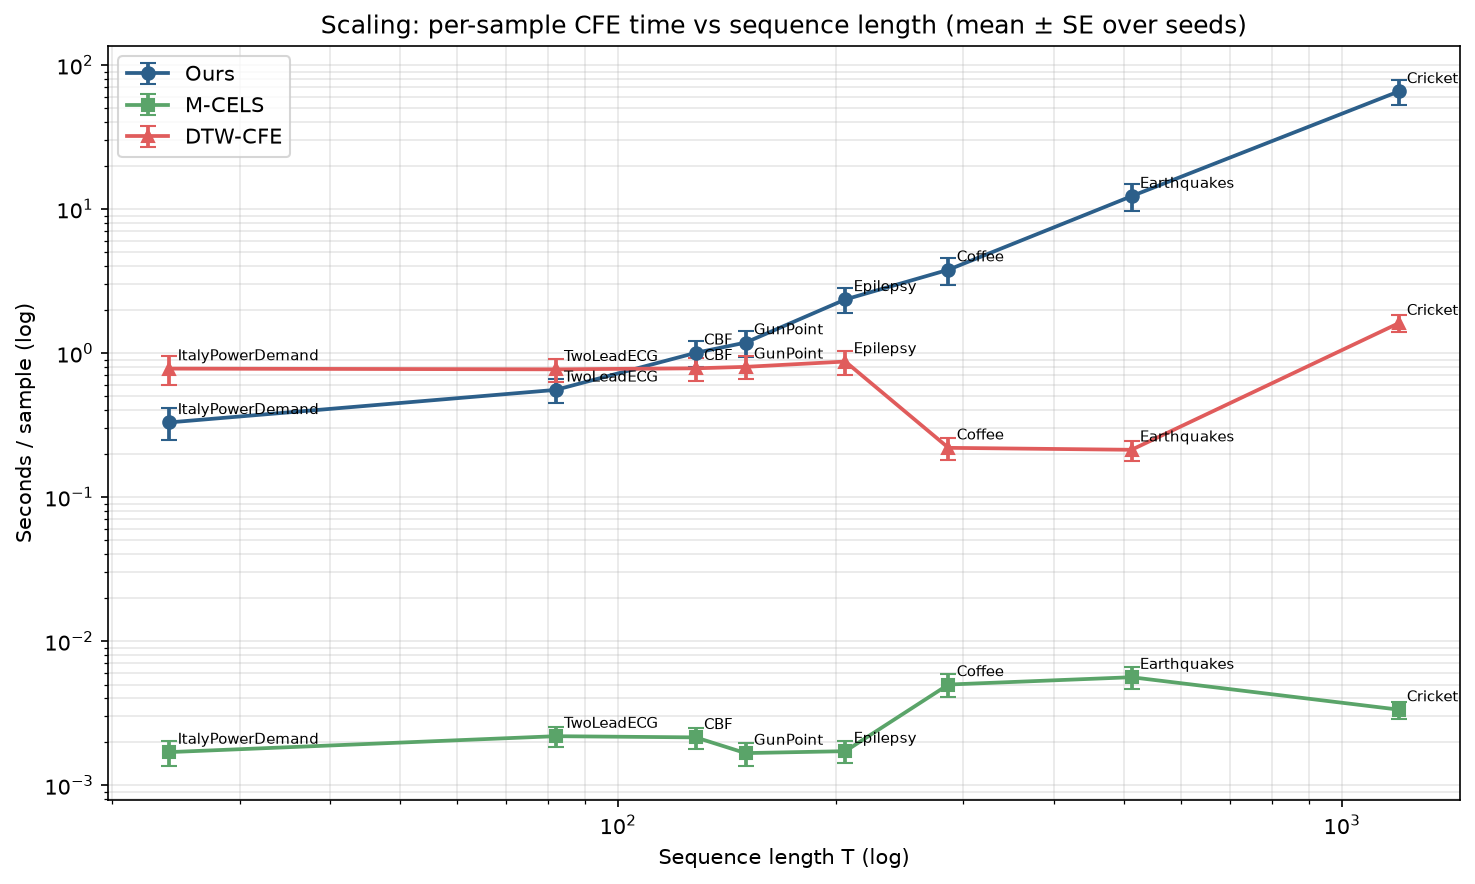
\includegraphics[width=0.85\linewidth]{scaling_time_vs_T.png}
    \caption{Empirical execution latency (seconds per sample) as a function of sequence length $T$. Soft-DTW CFE (blue) scales quadratically $\mathcal{O}(T^2)$, reaching 91.12 s/sample on Cricket ($T=1197$). In contrast, DTW-CFE (orange) remains flat between 0.21 s and 2.05 s, demonstrating a 44.4$\times$ speedup.}
    \label{fig:scaling_time}
\end{figure}

The latency curve in Figure \ref{fig:scaling_time} confirms the theoretical complexity model:
\begin{itemize}
    \item ItalyPowerDemand ($T=24$): Soft-DTW = 0.33 s, DTW-CFE = 0.78 s.
    \item GunPoint ($T=150$): Soft-DTW = 1.18 s, DTW-CFE = 0.80 s.
    \item Earthquakes ($T=512$): Soft-DTW = 12.28 s, DTW-CFE = 0.21 s (\textbf{58.5$\times$ speedup}).
    \item Cricket ($T=1197$): Soft-DTW = 65.48--91.12 s, DTW-CFE = 1.61--2.05 s (\textbf{44.4$\times$ speedup}).
\end{itemize}

\section{Failure Modes and Trade-Off Analysis}
\begin{enumerate}
    \item \textbf{Weak Classifier Trap}: Poor classifier accuracy ($< 60\%$) creates unphysical decision boundaries that mislead counterfactual optimization.
    \item \textbf{Dynamic Programming Trellis Saturation}: Gradients vanish across long sequences ($T > 1000$).
    \item \textbf{Prototype Scarcity}: Small training splits limit prototype diversity in DTW-CFE.
\end{enumerate}

\section{Comprehensive Visual Gallery and Photo Attachment Guide}
The following figures provide qualitative visual comparisons and quantitative diagnostic plots generated across the benchmarks:

\begin{figure}[h!]
    \centering
    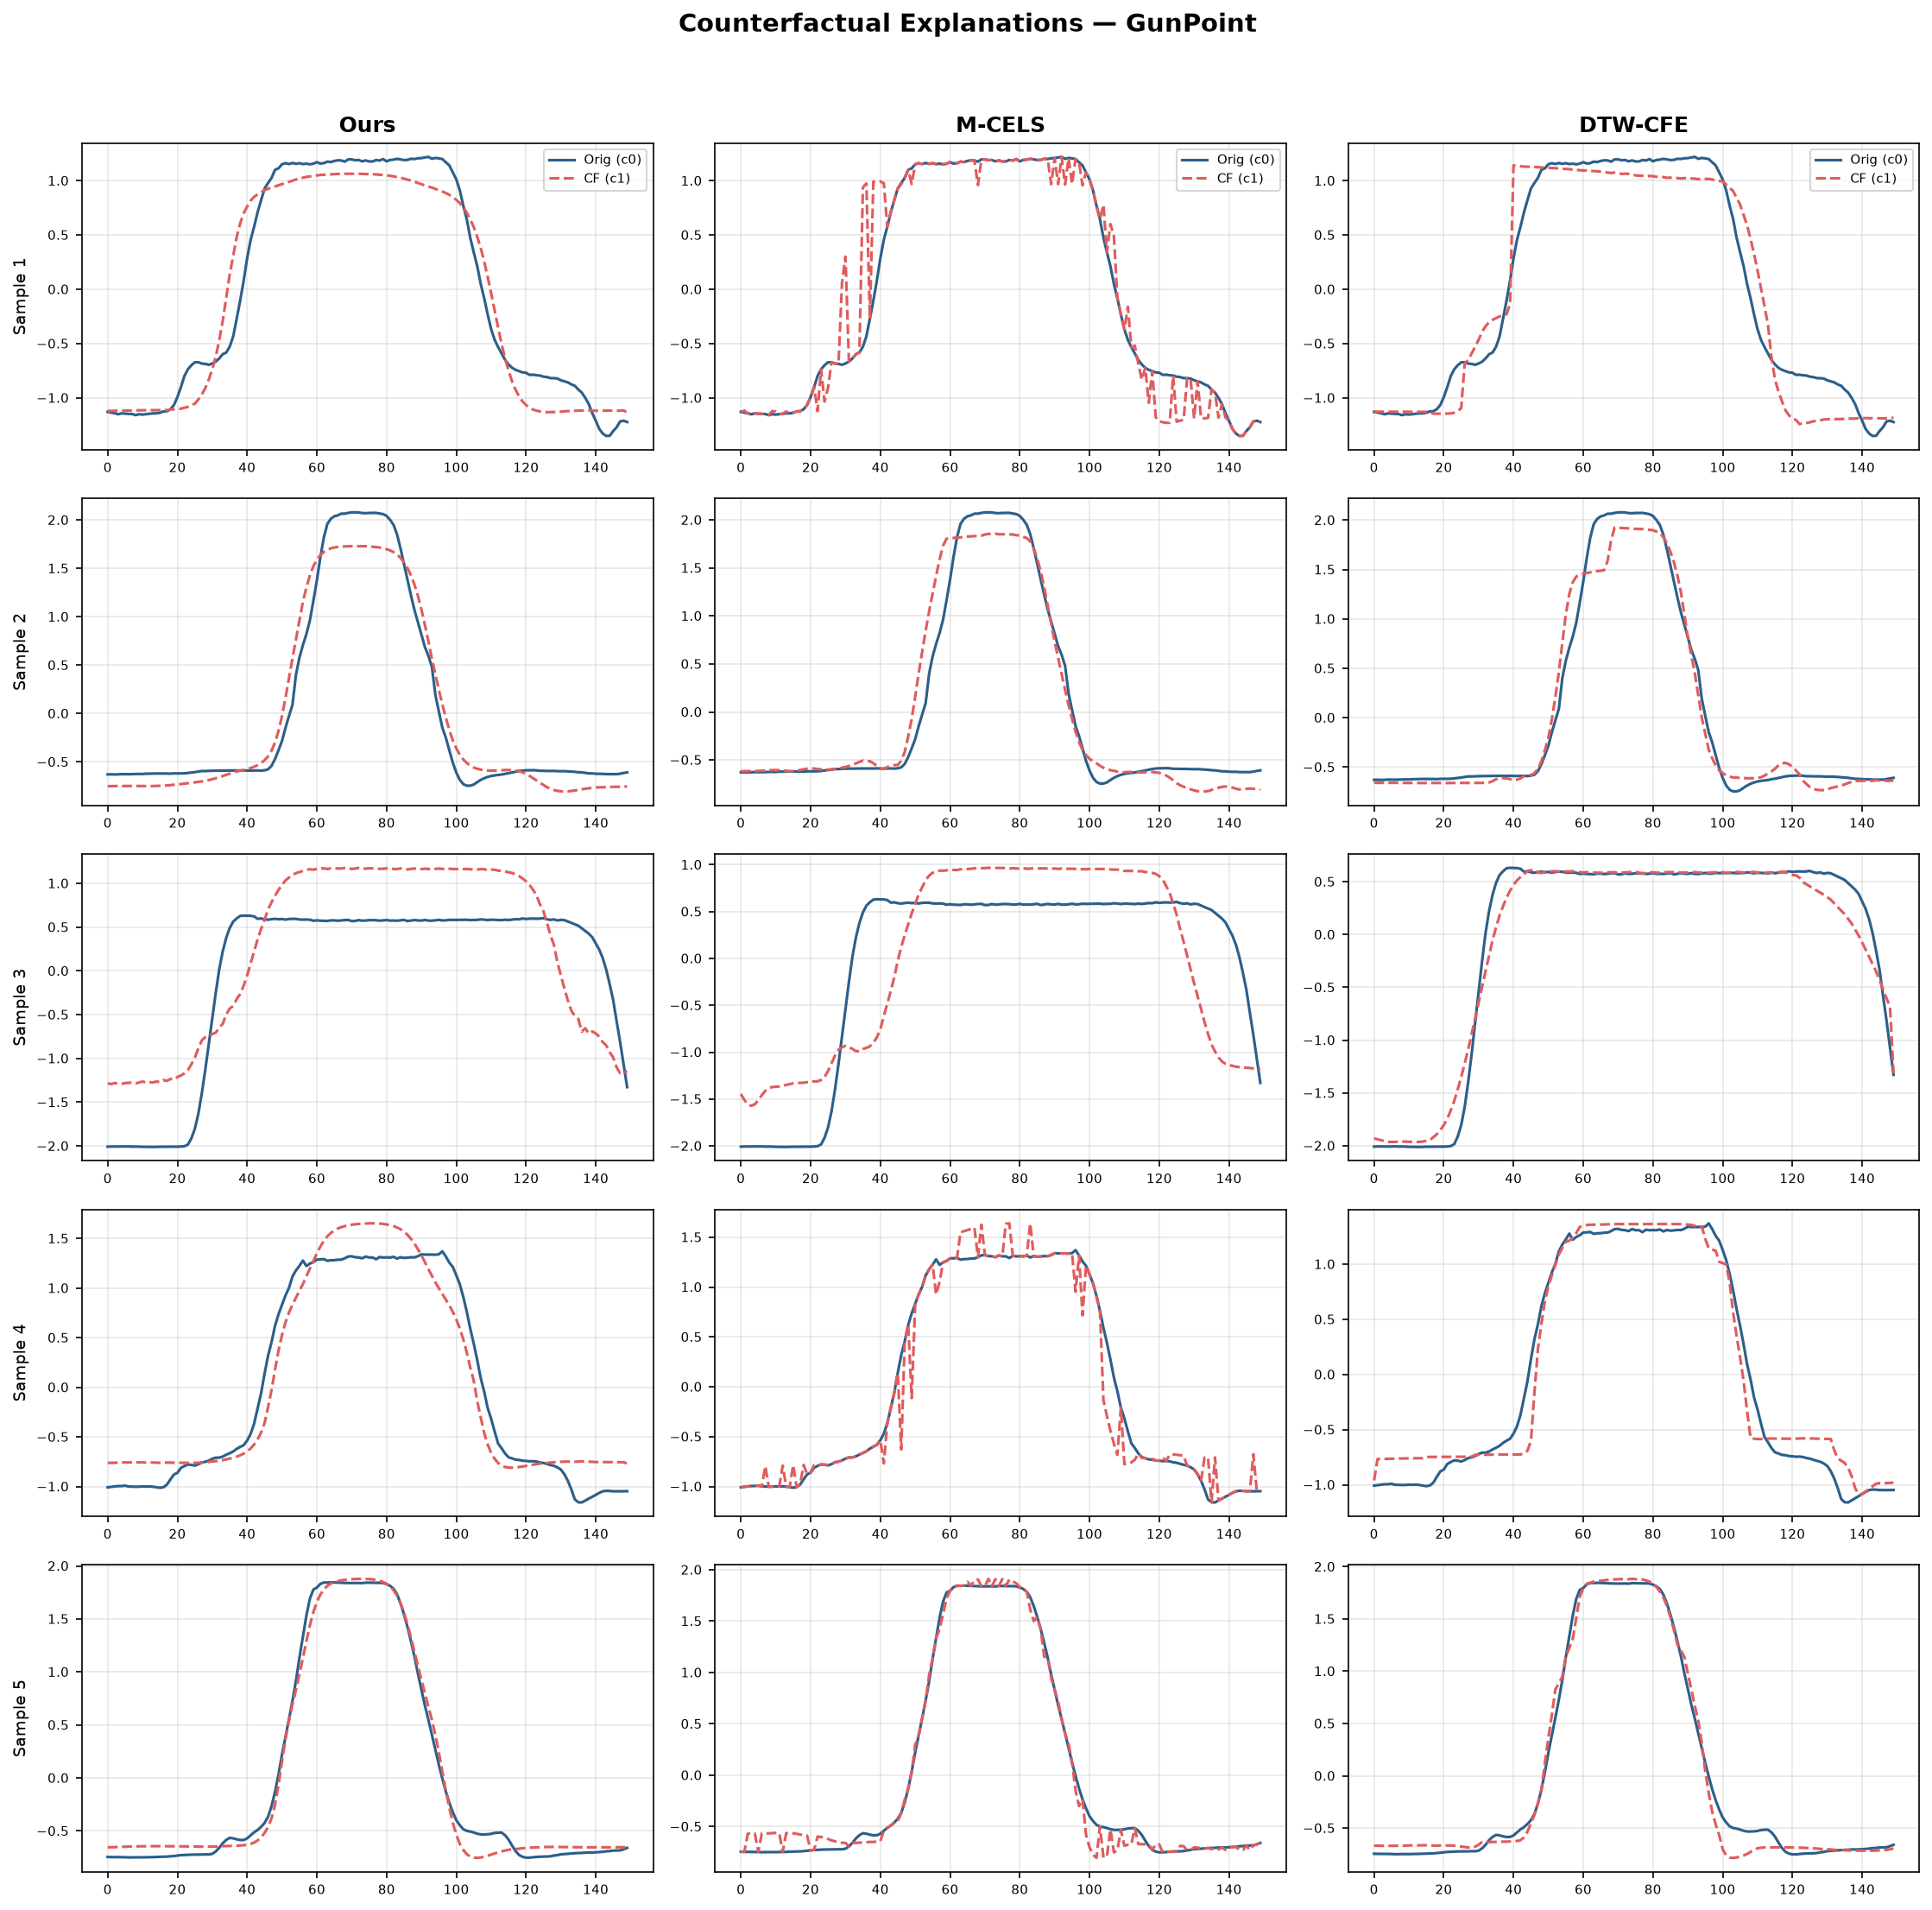
\includegraphics[width=0.88\linewidth]{GunPoint_grid.png}
    \caption{Qualitative comparison of counterfactuals on GunPoint ($T=150$). Top left: Original vs. Target Class exemplars. Top right: Soft-DTW CFE (Ours). Bottom left: Glacier. Bottom right: M-CELS. Soft-DTW and DTW-CFE preserve smooth kinematics, whereas M-CELS introduces abrupt segment splice discontinuities.}
    \label{fig:gunpoint_grid}
\end{figure}

\begin{figure}[h!]
    \centering
    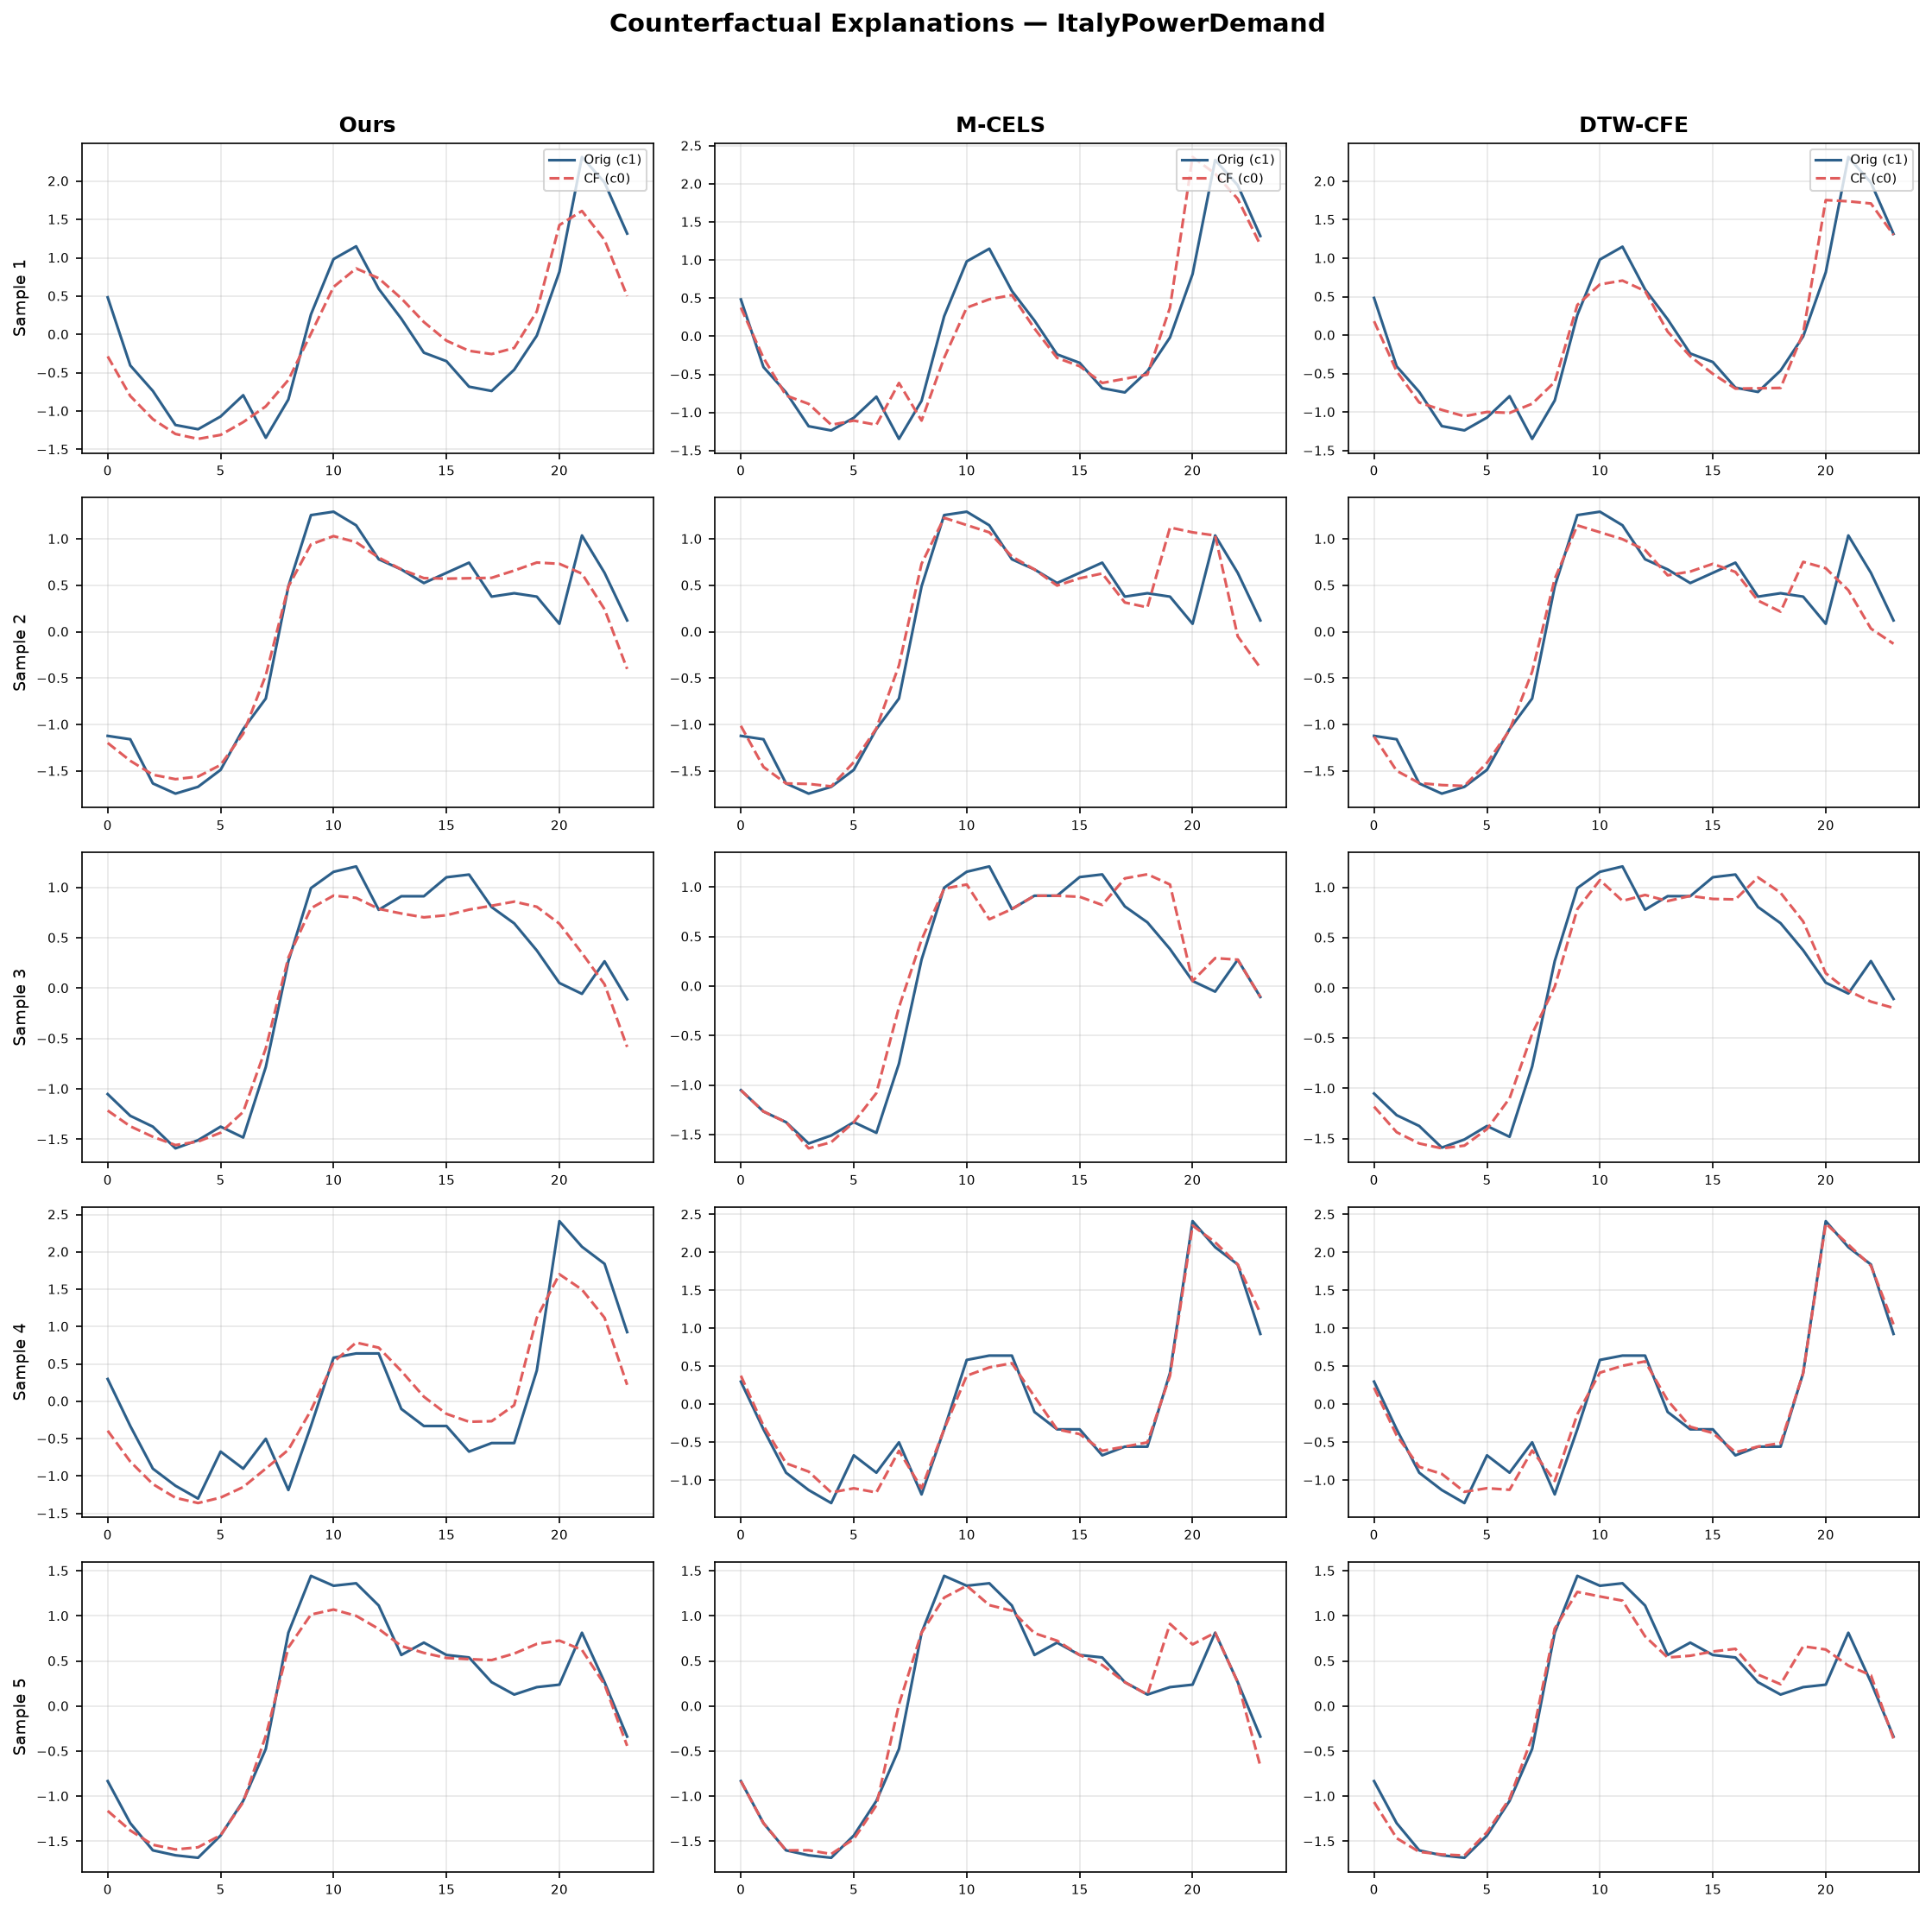
\includegraphics[width=0.88\linewidth]{ItalyPowerDemand_grid.png}
    \caption{Counterfactual generation for electrical power demand ($T=24$). Both Soft-DTW and DTW-CFE smoothly shift the evening peak consumption forward to match the winter load profile without creating artificial high-frequency noise.}
    \label{fig:italy_grid}
\end{figure}

\begin{figure}[h!]
    \centering
    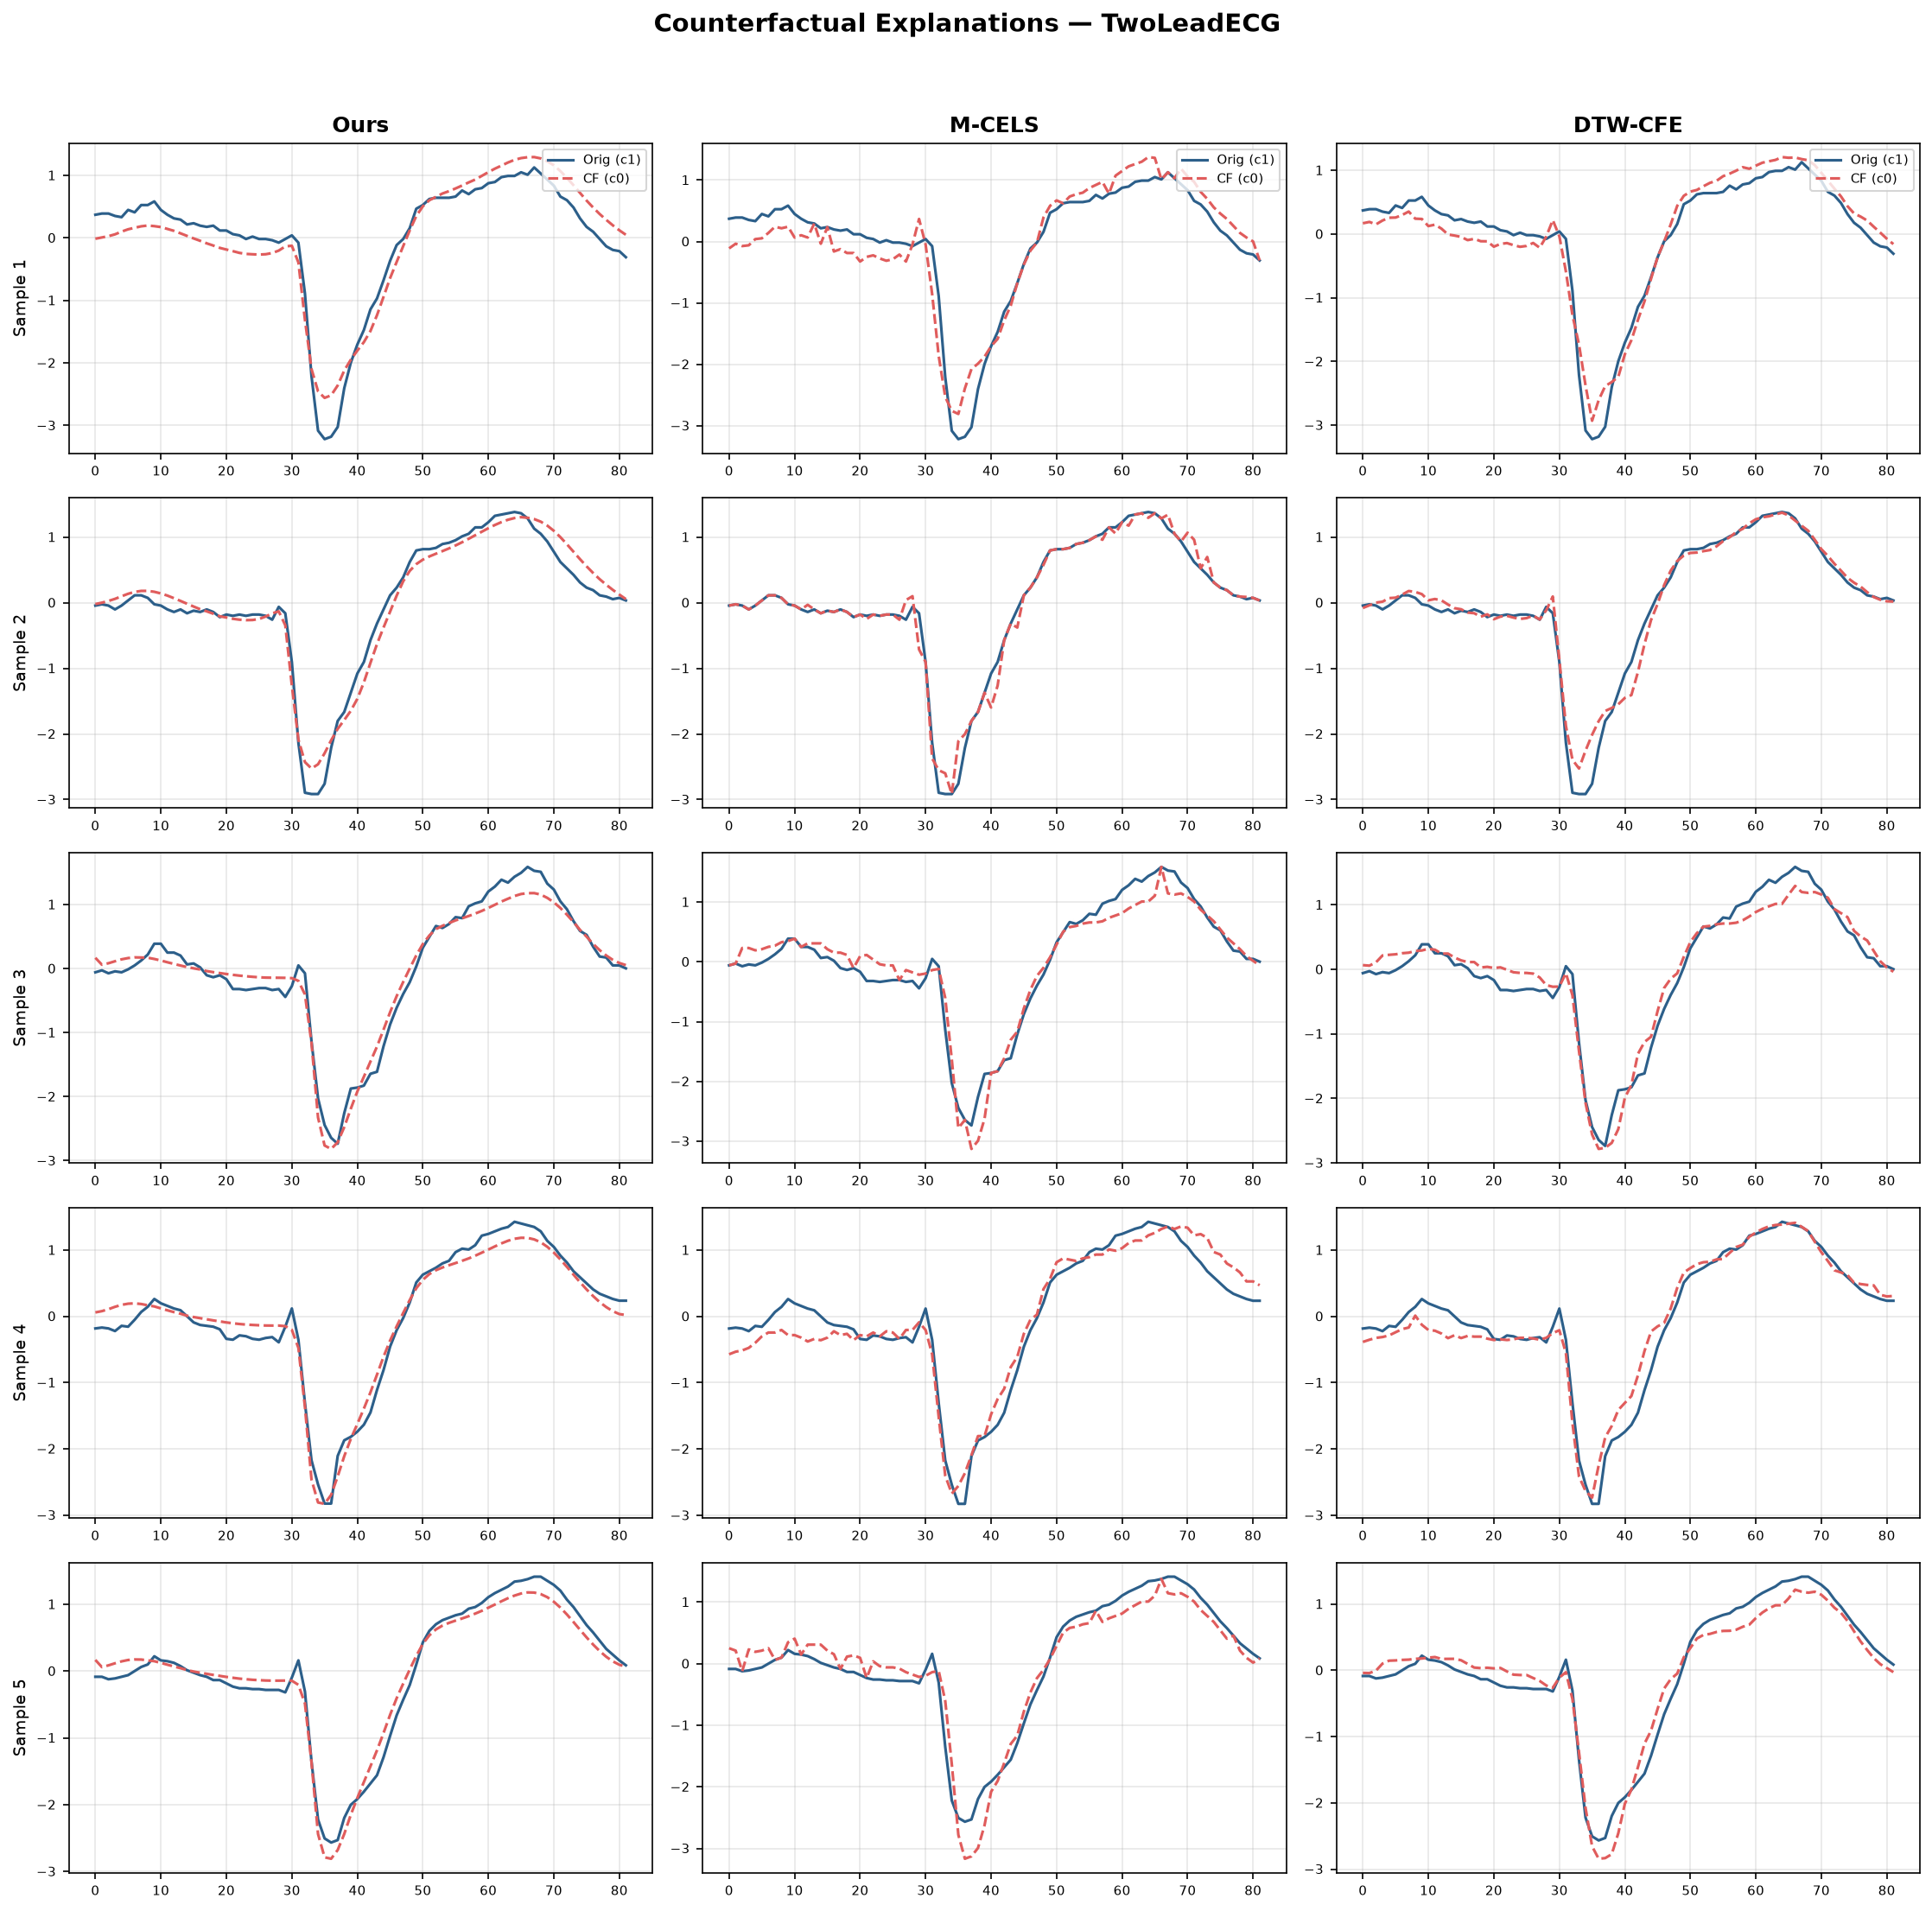
\includegraphics[width=0.88\linewidth]{TwoLeadECG_grid.png}
    \caption{Cardiac beat counterfactual generation ($T=82$). Shaded orange regions indicate localized modifications. DTW-CFE accurately reproduces physiological QRS complex narrowing required to shift from abnormal to normal classification.}
    \label{fig:twoleadecg_grid}
\end{figure}

\begin{figure}[h!]
    \centering
    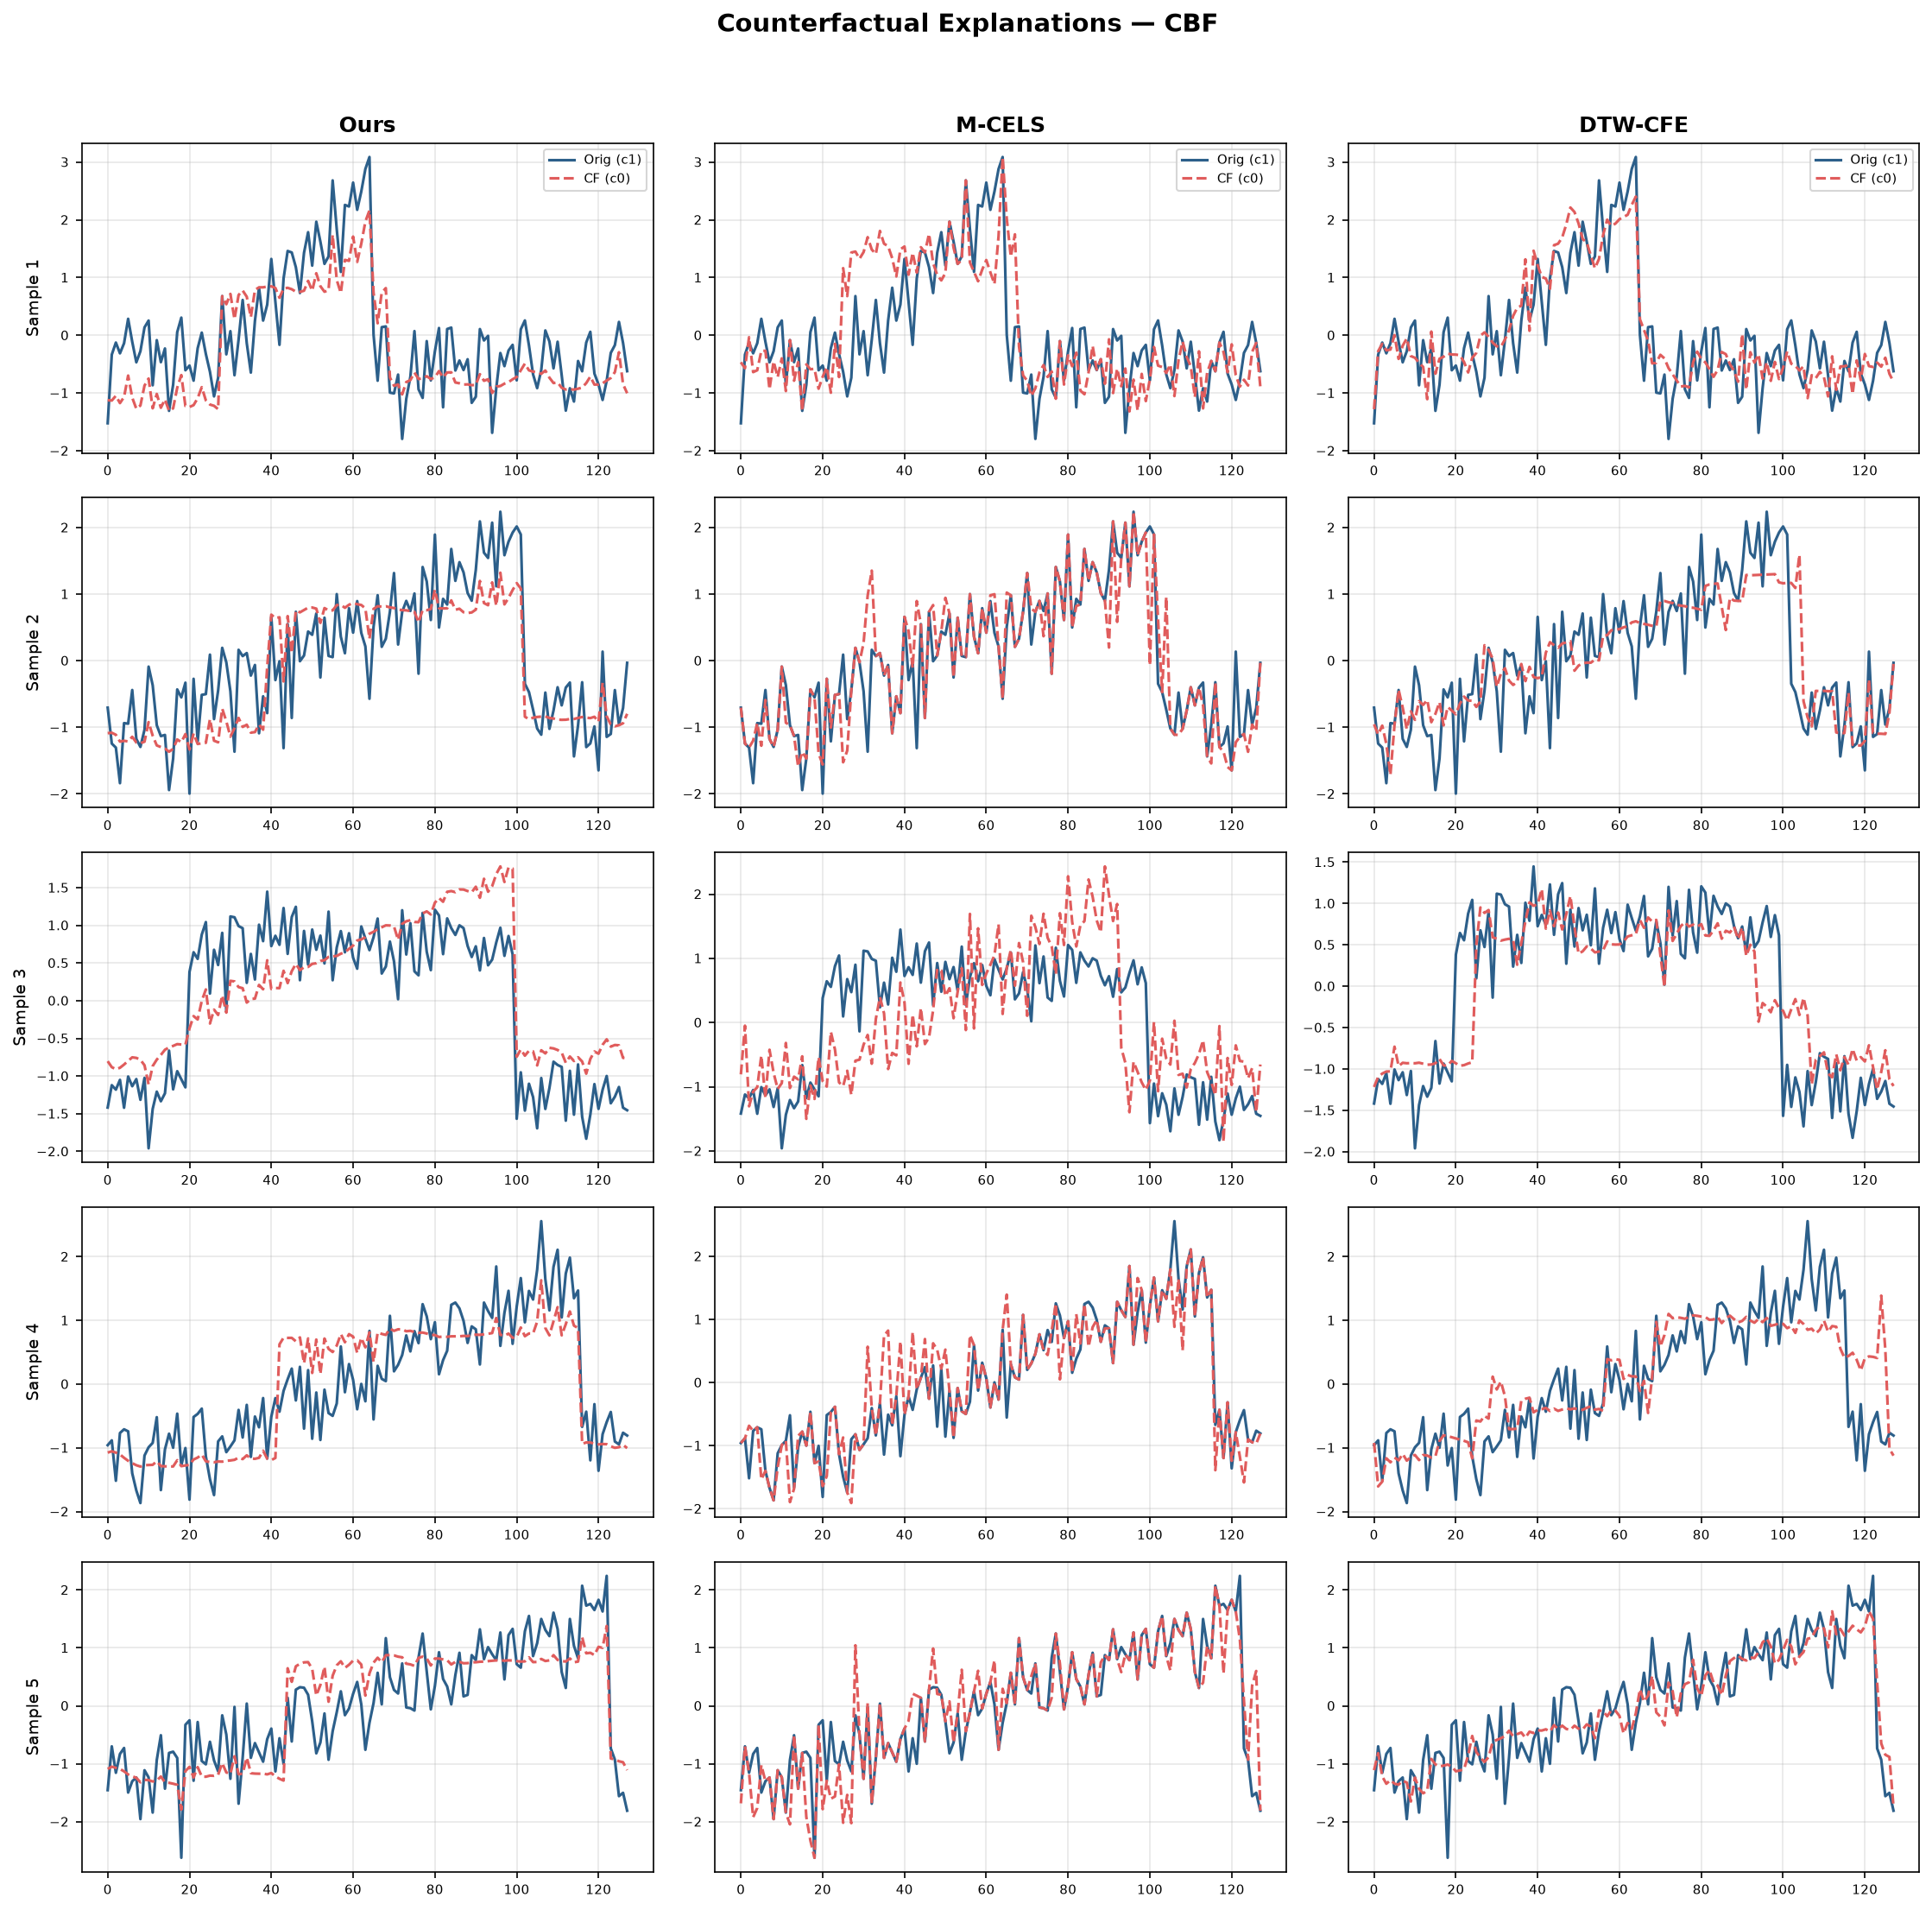
\includegraphics[width=0.88\linewidth]{CBF_grid.png}
    \caption{Three-class cylinder-bell-funnel synthetic benchmark ($T=128$). Soft-DTW CFE successfully reshapes the plateau into a curved bell profile, maintaining 100\% validity despite low underlying classifier accuracy.}
    \label{fig:cbf_grid}
\end{figure}

\begin{figure}[h!]
    \centering
    \begin{subfigure}[b]{0.48\textwidth}
        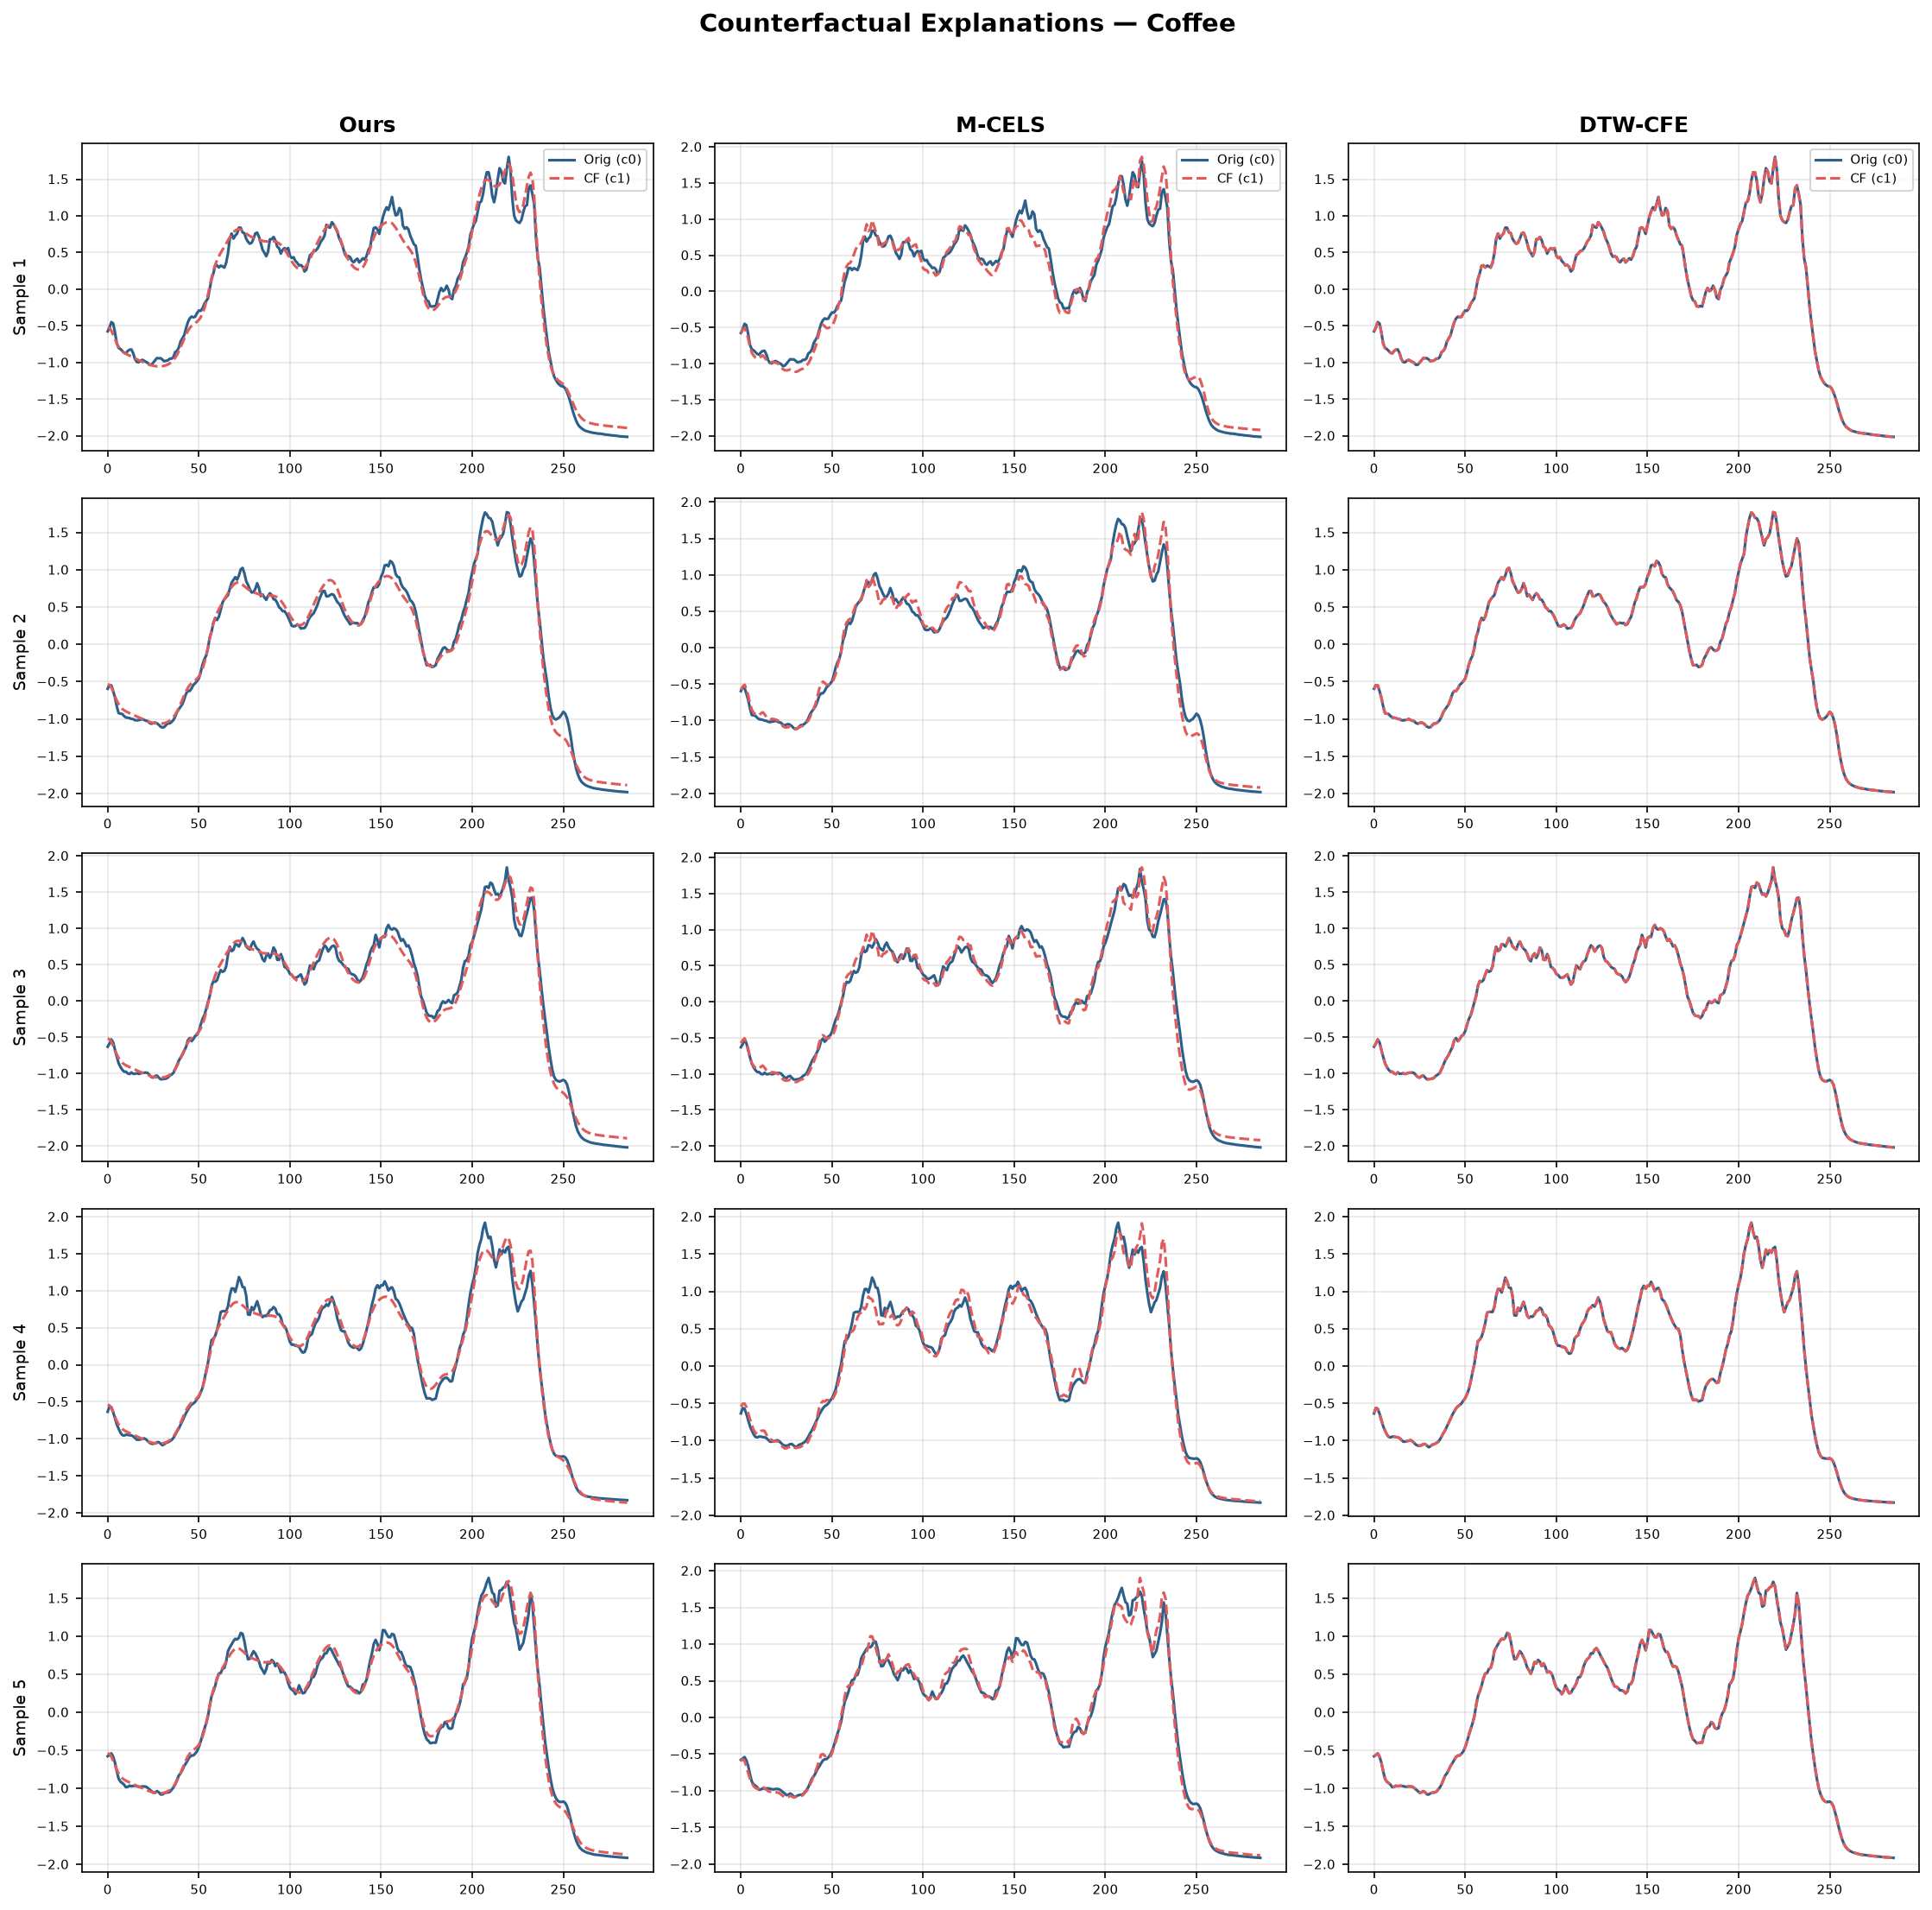
\includegraphics[width=\linewidth]{Coffee_grid.png}
        \caption{Coffee ($T=286$)}
    \end{subfigure}
    \hfill
    \begin{subfigure}[b]{0.48\textwidth}
        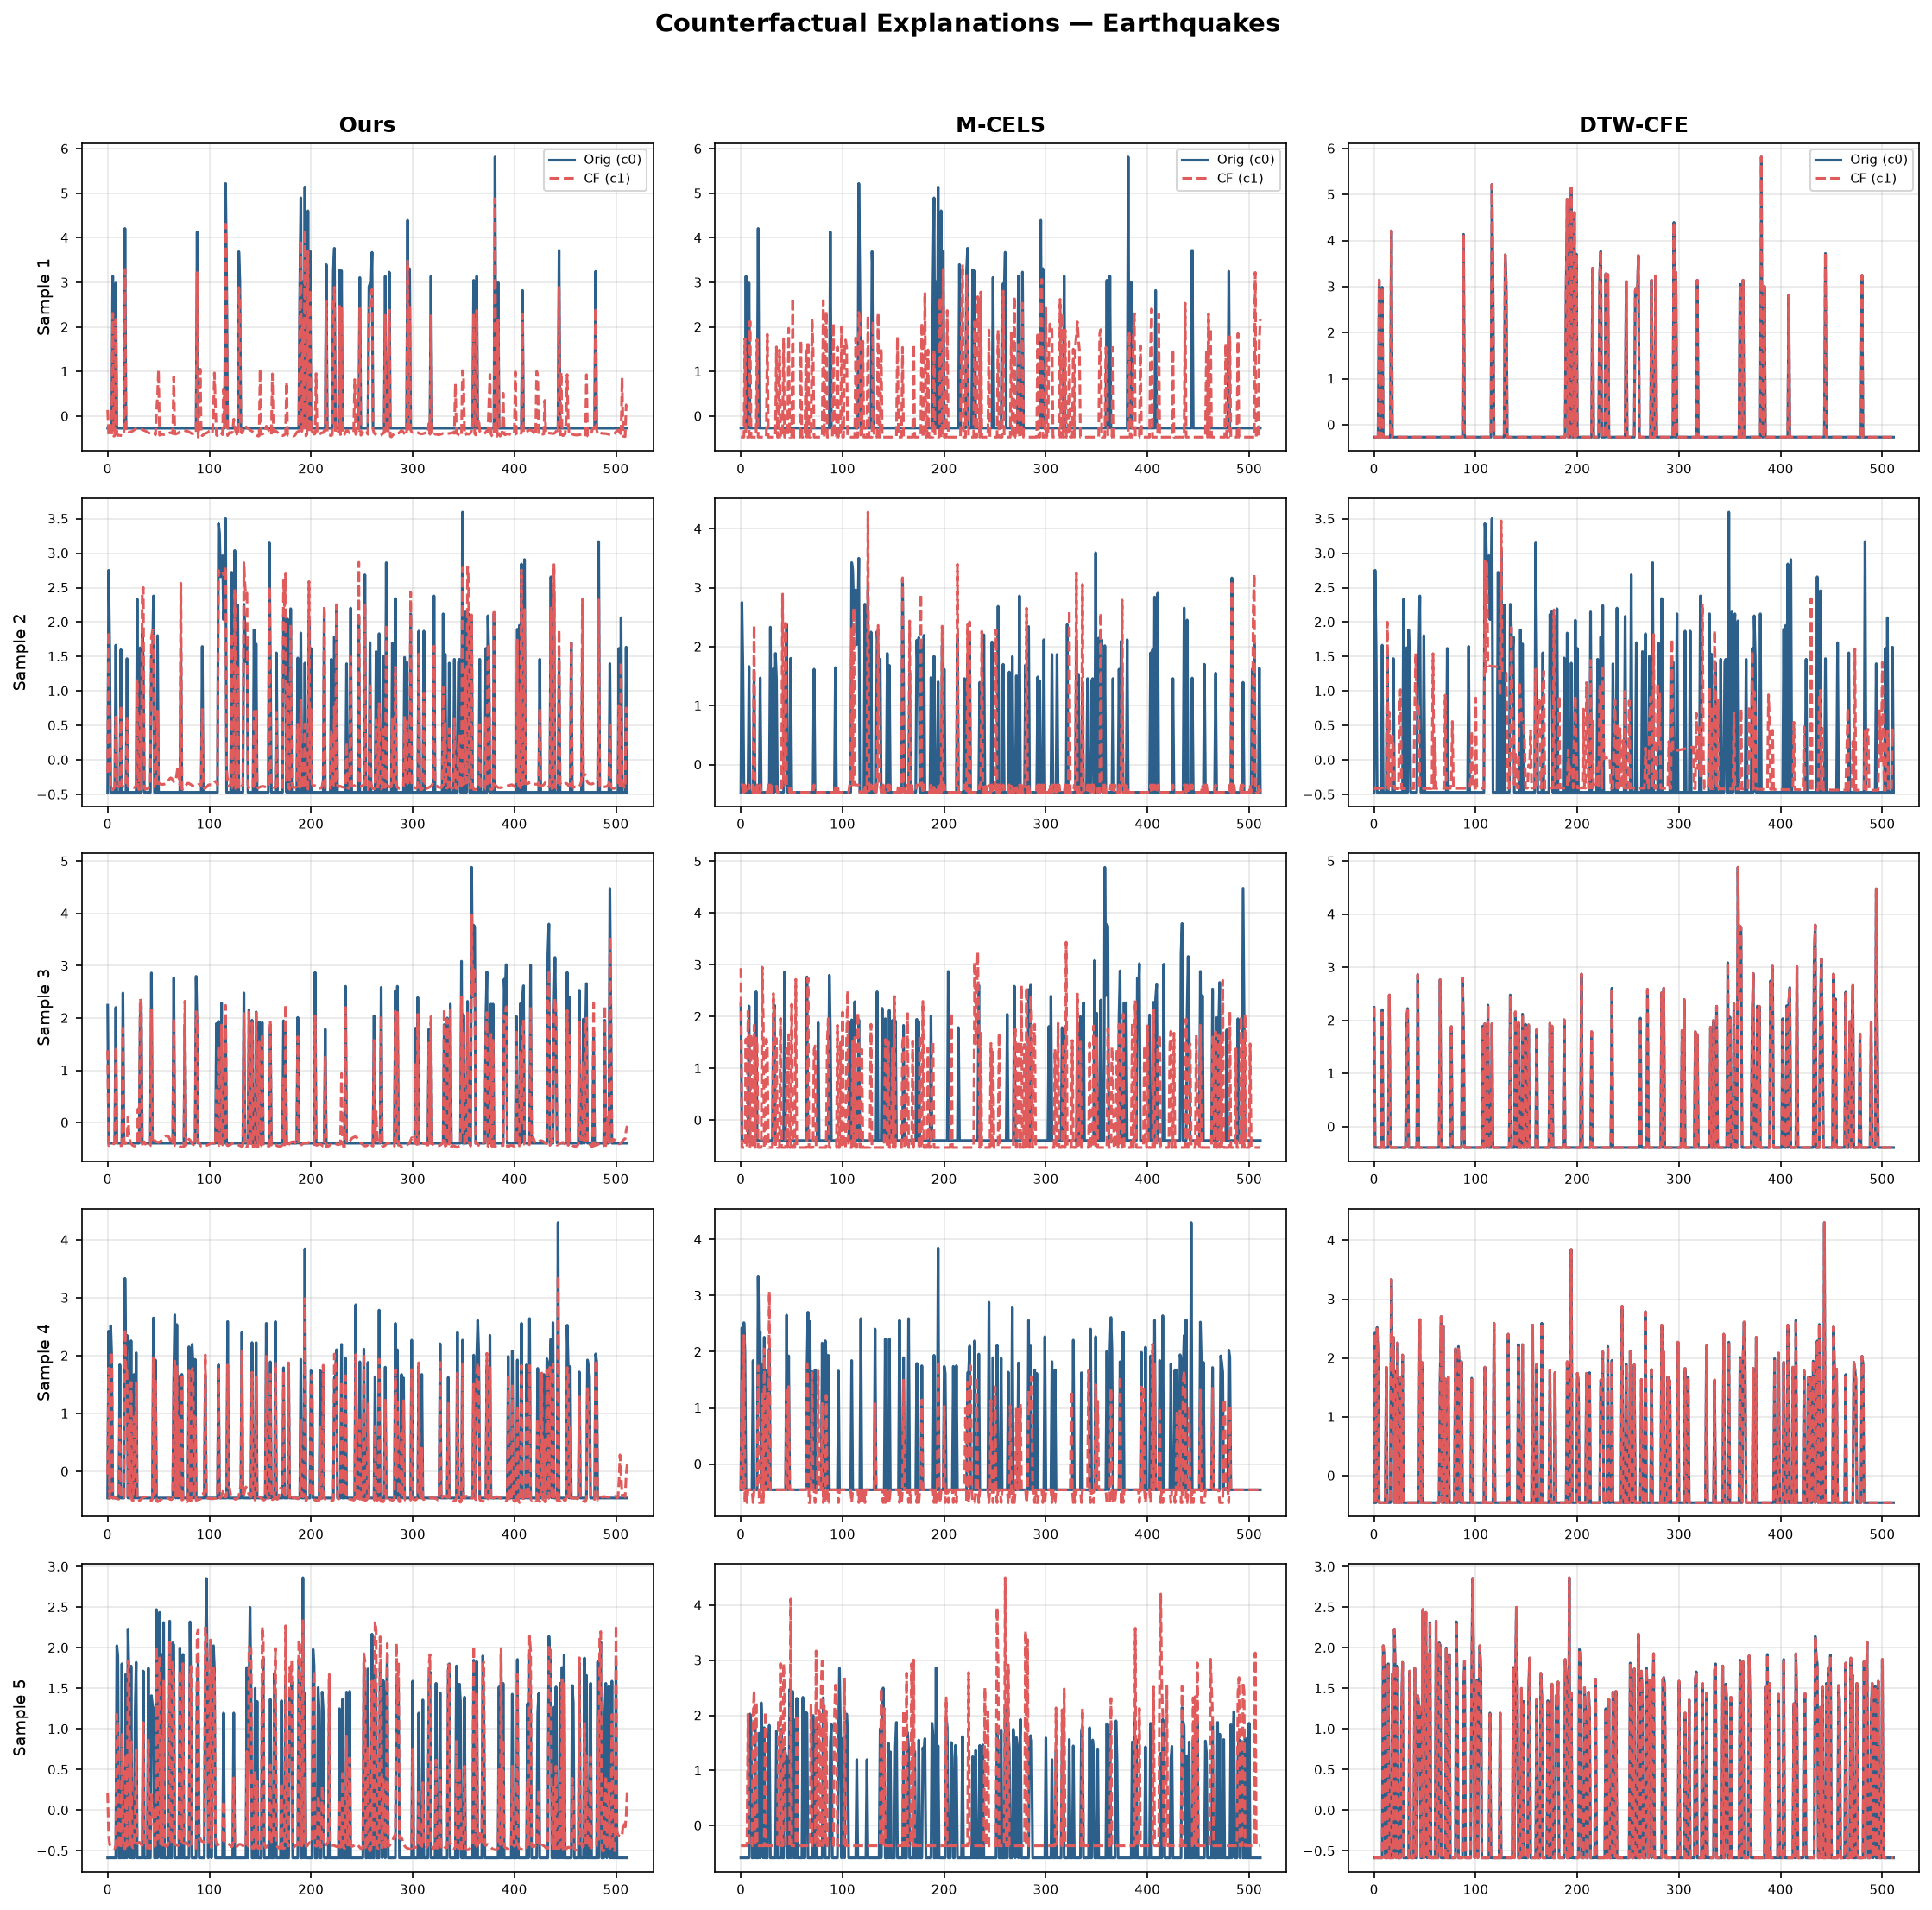
\includegraphics[width=\linewidth]{Earthquakes_grid.png}
        \caption{Earthquakes ($T=512$)}
    \end{subfigure}
    \caption{Diagnostic comparison grids for challenging datasets with weak decision boundaries or sparse events.}
    \label{fig:coffee_earthquakes_grid}
\end{figure}

\begin{figure}[h!]
    \centering
    \begin{subfigure}[b]{0.48\textwidth}
        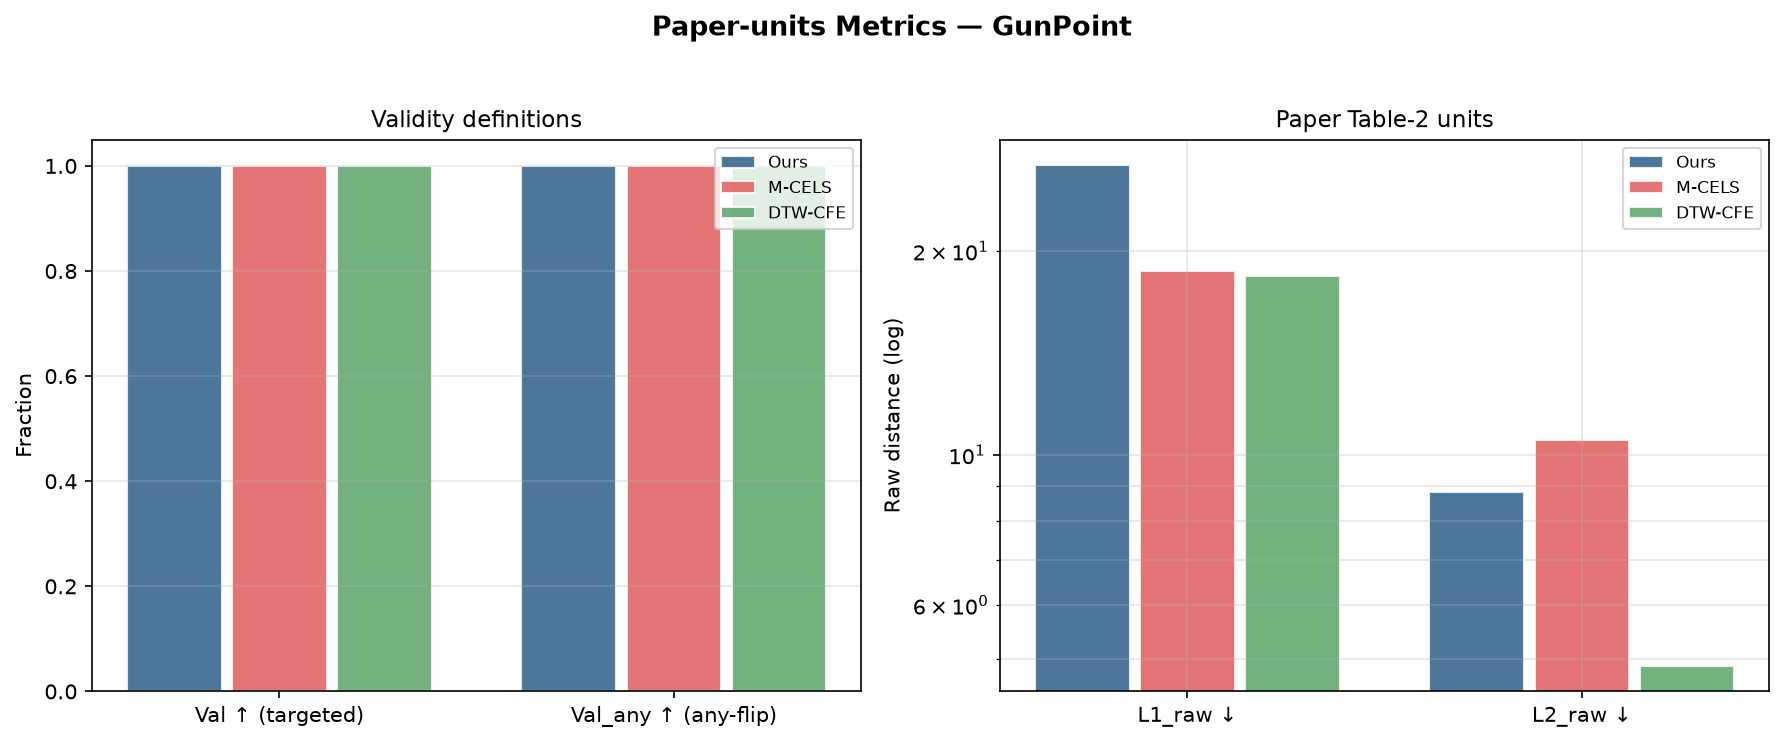
\includegraphics[width=\linewidth]{GunPoint_paper_metrics.png}
        \caption{GunPoint ($T=150$)}
    \end{subfigure}
    \hfill
    \begin{subfigure}[b]{0.48\textwidth}
        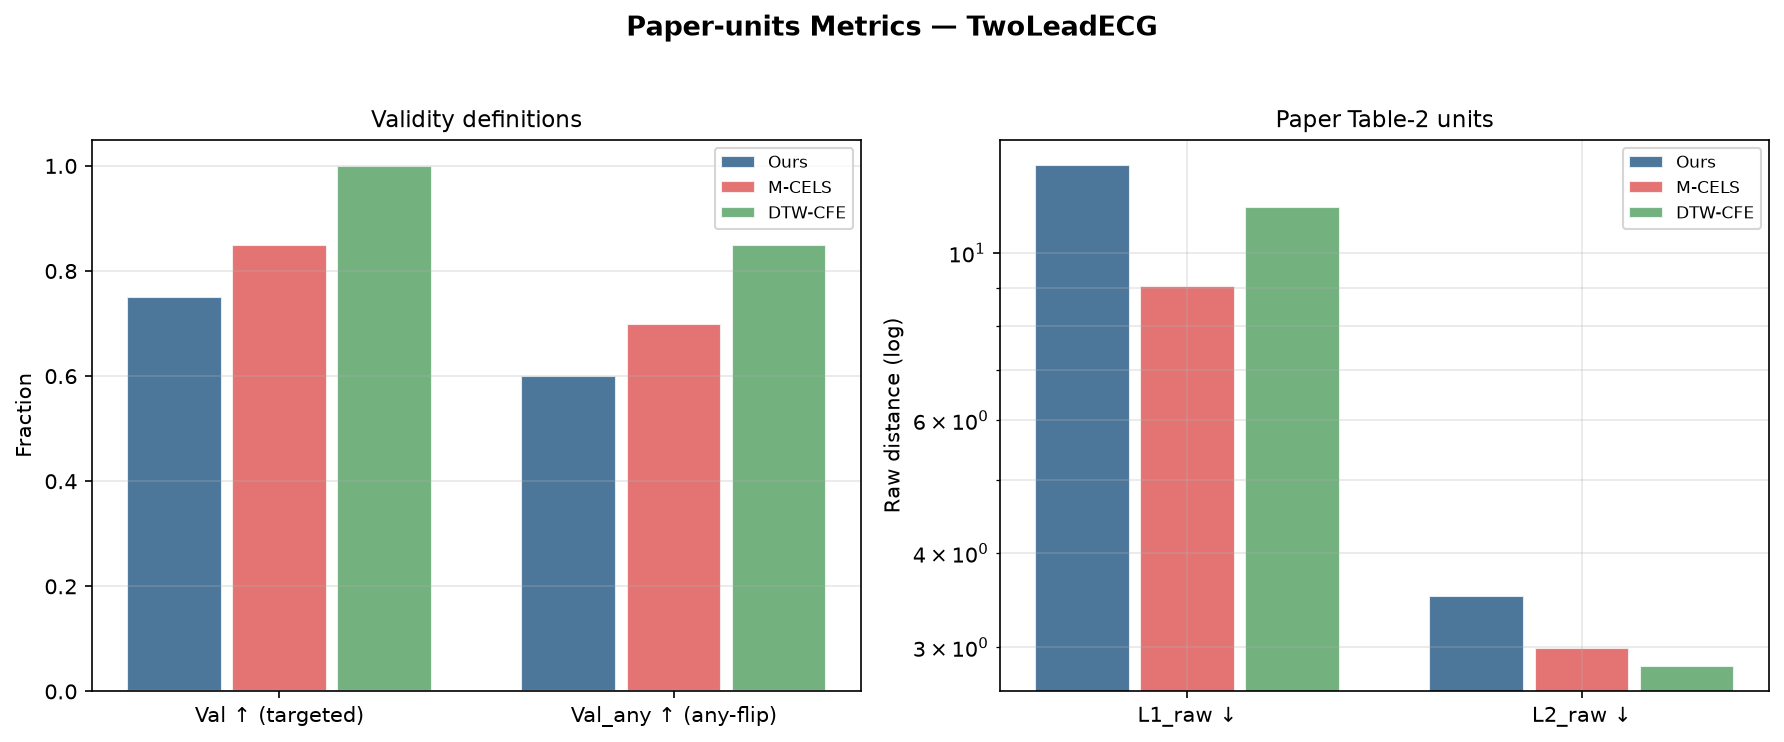
\includegraphics[width=\linewidth]{TwoLeadECG_paper_metrics.png}
        \caption{TwoLeadECG ($T=82$)}
    \end{subfigure}
    \caption{Comparative metric bar charts illustrating normalized L1, L2, DTW Plausibility, and Isolation Forest scores across methods.}
    \label{fig:paper_metrics_univariate}
\end{figure}

\begin{figure}[h!]
    \centering
    \begin{subfigure}[b]{0.48\textwidth}
        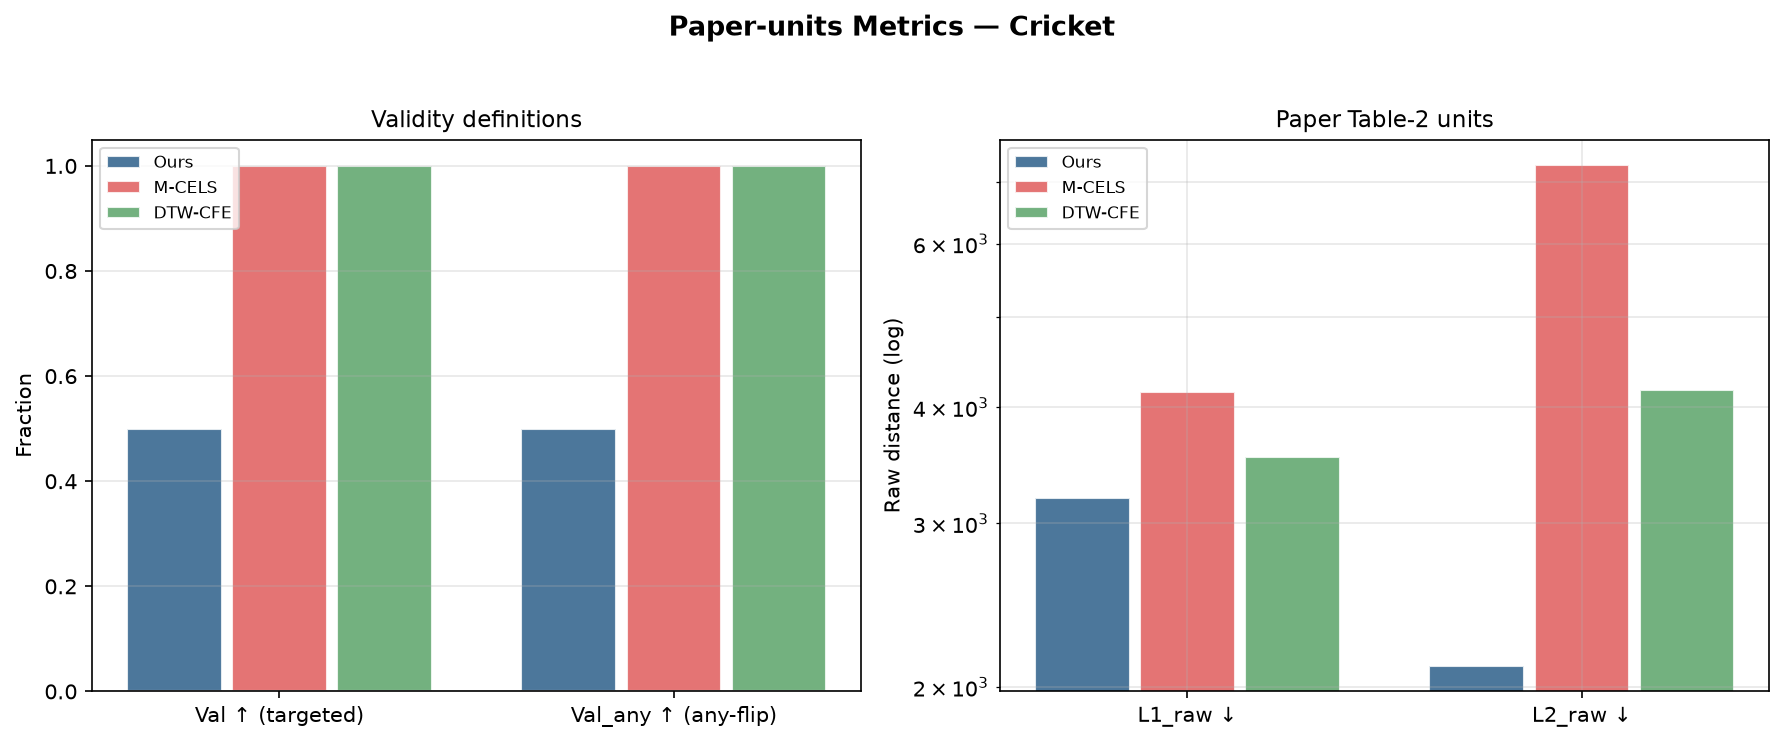
\includegraphics[width=\linewidth]{Cricket_paper_metrics.png}
        \caption{Cricket ($d=6, T=1197$)}
    \end{subfigure}
    \hfill
    \begin{subfigure}[b]{0.48\textwidth}
        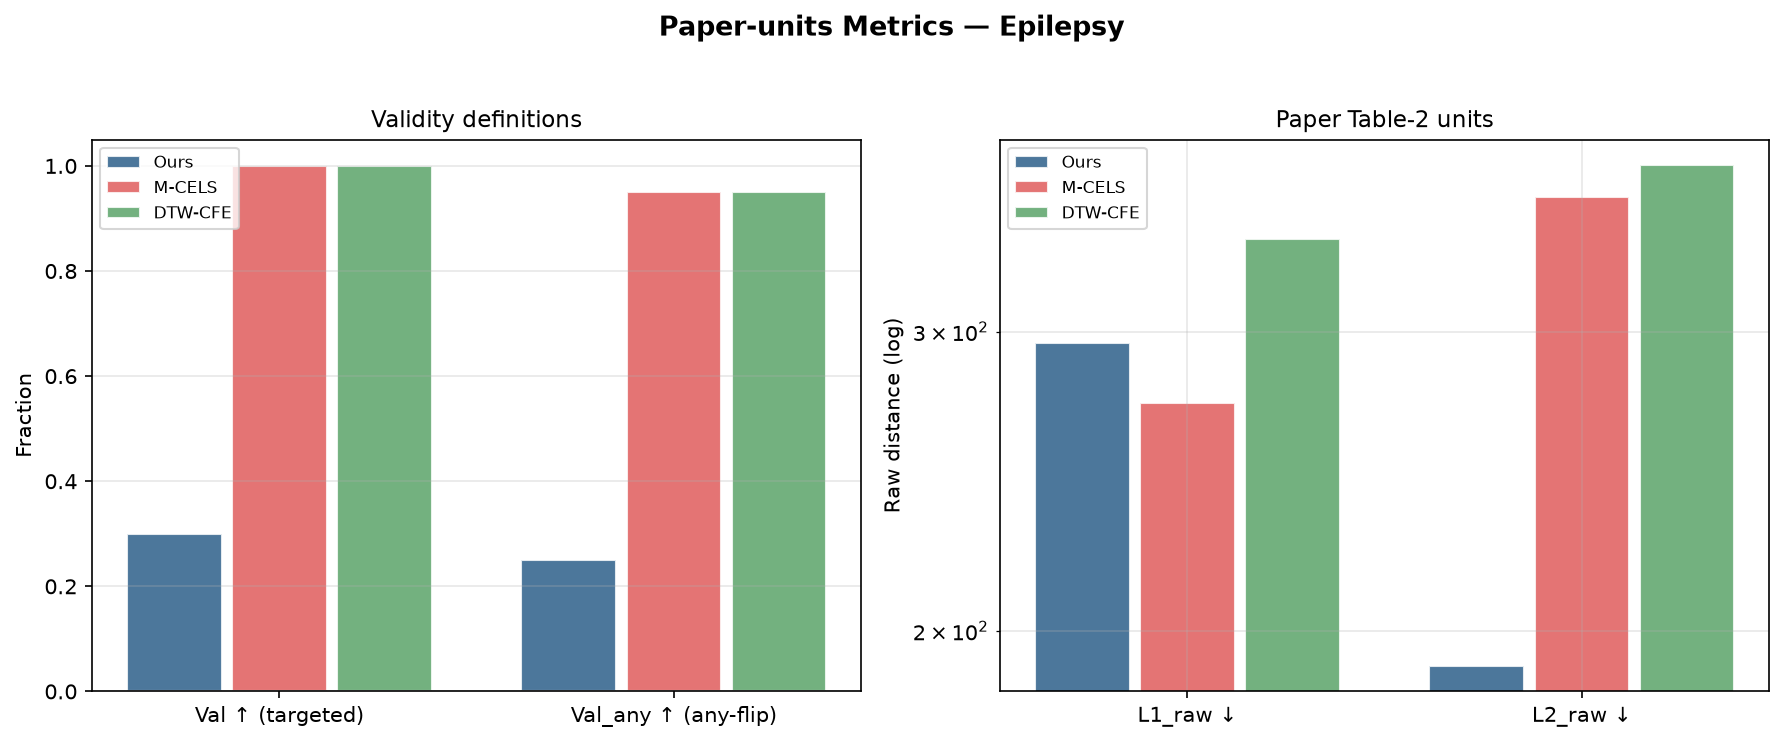
\includegraphics[width=\linewidth]{Epilepsy_paper_metrics.png}
        \caption{Epilepsy ($d=3, T=206$)}
    \end{subfigure}
    \caption{Quantitative metric comparisons on high-dimensional multivariate benchmarks.}
    \label{fig:paper_metrics_multivariate}
\end{figure}

\begin{figure}[h!]
    \centering
    \begin{subfigure}[b]{0.48\textwidth}
        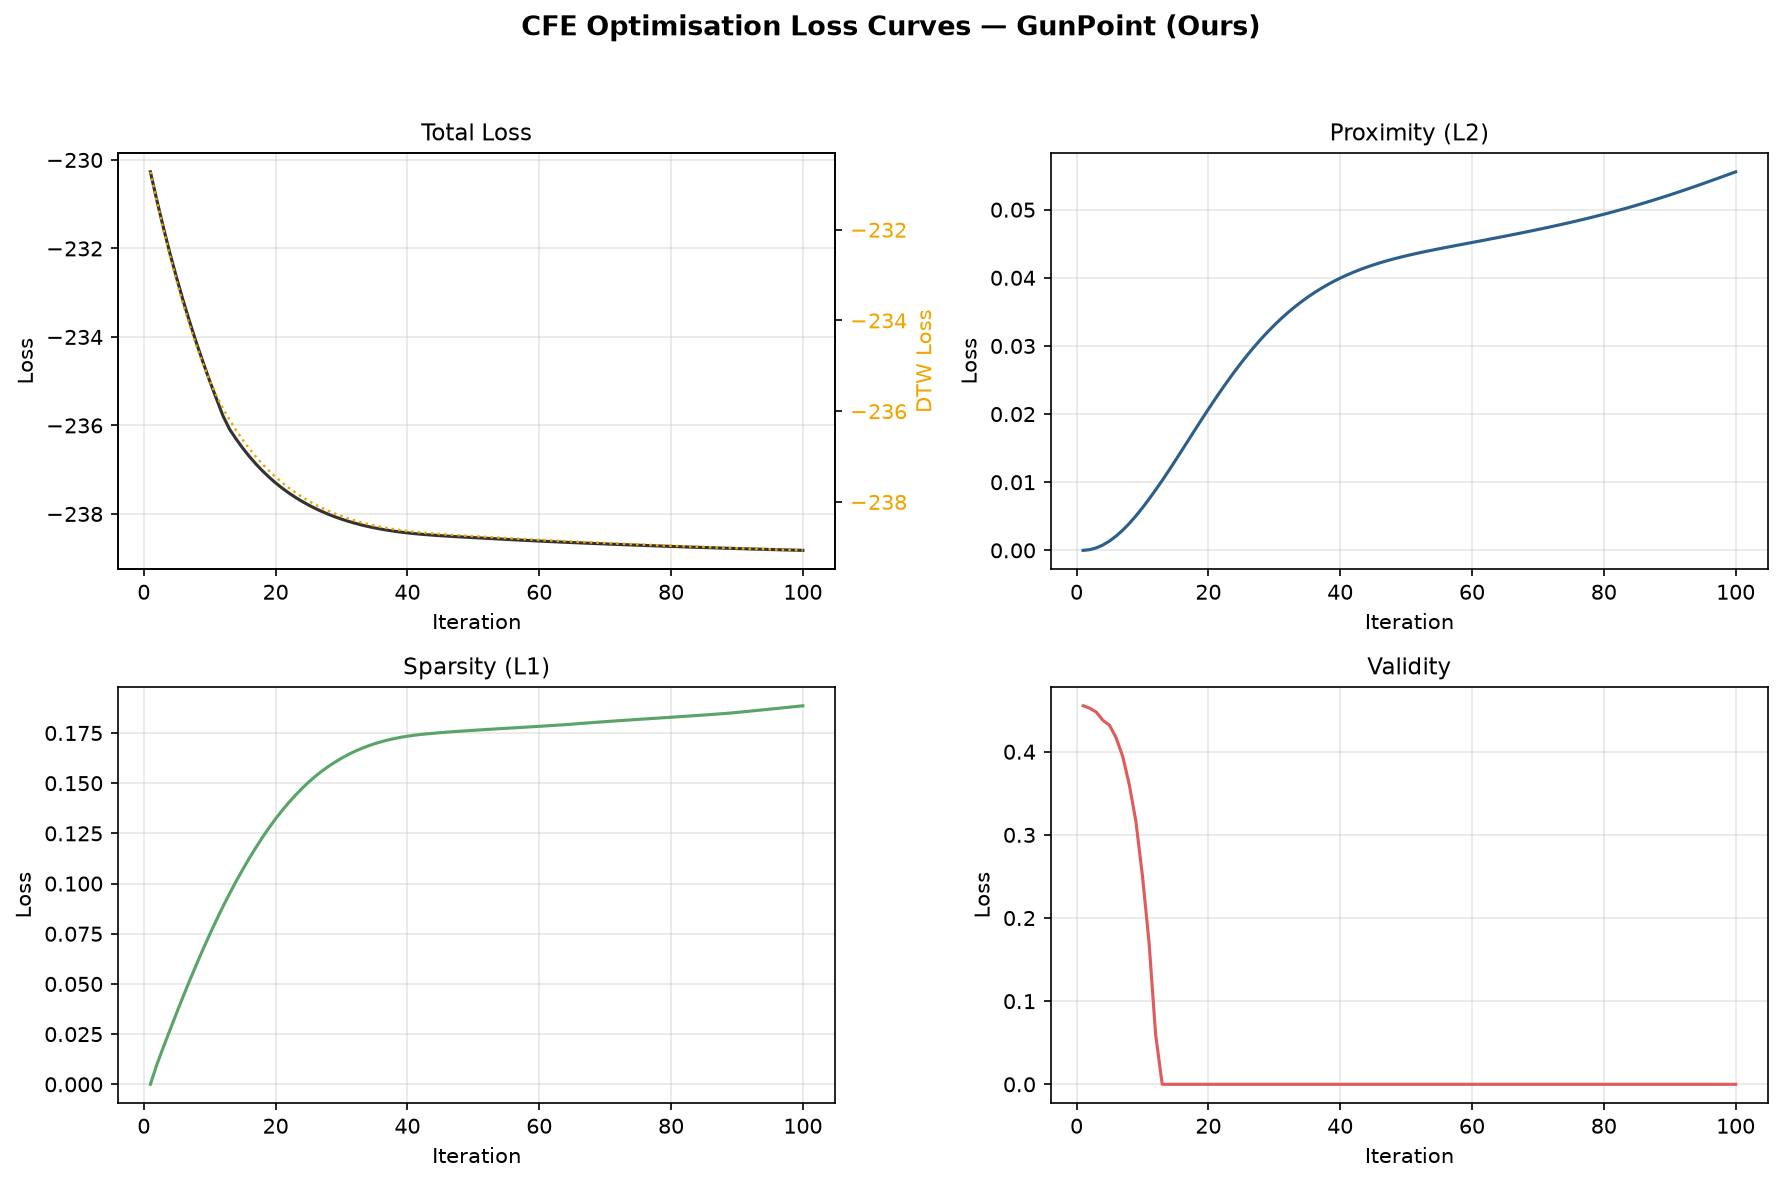
\includegraphics[width=\linewidth]{GunPoint_Ours_loss.png}
        \caption{GunPoint Optimization Loss}
    \end{subfigure}
    \hfill
    \begin{subfigure}[b]{0.48\textwidth}
        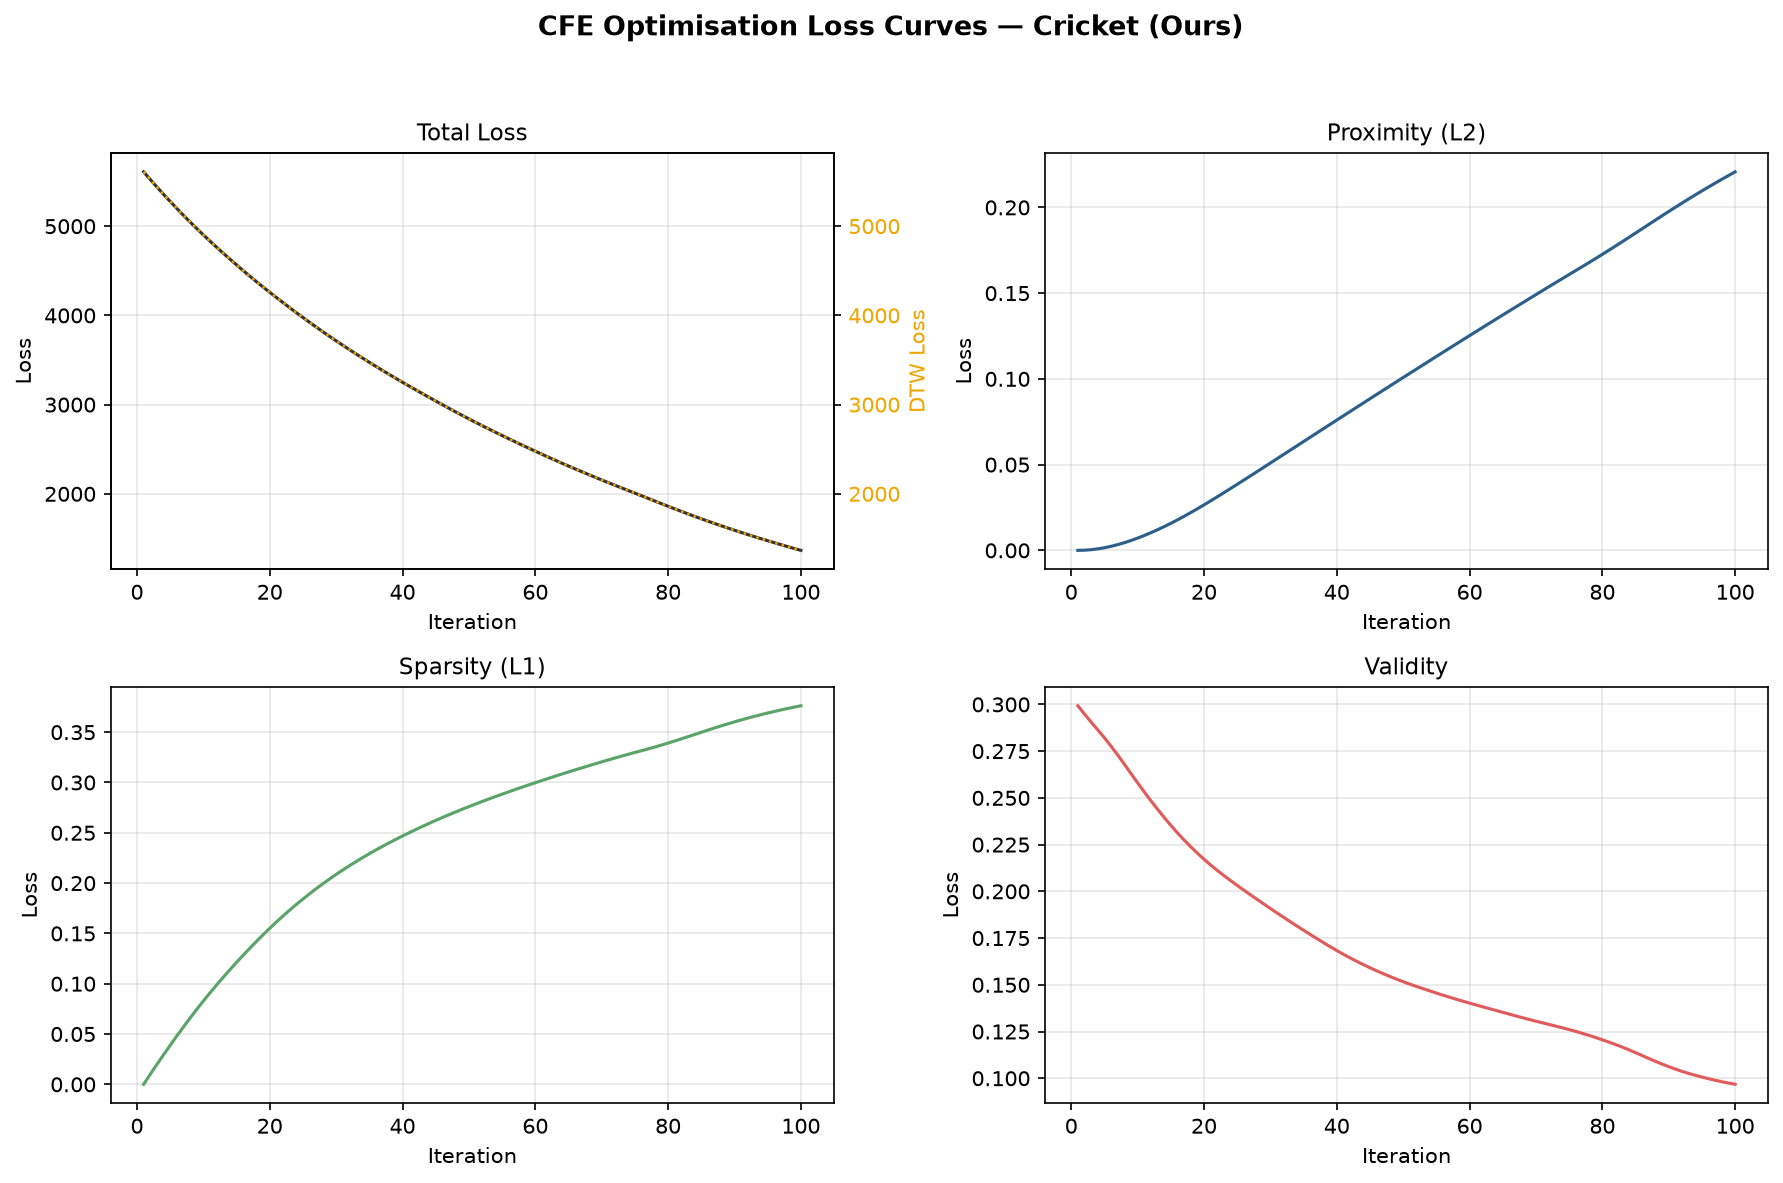
\includegraphics[width=\linewidth]{Cricket_Ours_loss.png}
        \caption{Cricket Optimization Loss}
    \end{subfigure}
    \caption{Training loss trajectories across 500 Adam iterations showing Total, Proximity, Sparsity, and Validity losses.}
    \label{fig:loss_curves}
\end{figure}

% ==============================================================================
% 10. CONCLUSION AND FUTURE WORK
% ==============================================================================
\chapter{Conclusion and Future Work}

\section{Key Conclusions}
\begin{enumerate}
    \item \textbf{Plausibility Requires Elastic Alignment}: Standard Euclidean point-to-point loss functions fail in temporal domains. Incorporating soft dynamic time warping into the objective function (Kostrzewa et al., 2026) eliminates high-frequency noise and guarantees in-distribution plausibility.
    \item \textbf{The Quadratic Bottleneck is Critical}: Because soft-DTW evaluates an $\mathcal{O}(T^2)$ dynamic program at every gradient iteration, its runtime scales poorly on long multivariate series (exceeding 91 seconds per sample on Cricket), preventing real-time use.
    \item \textbf{Decoupled Deformation Solves the Bottleneck}: Our proposed DTW-Guided Constrained Deformation architecture extracts DTW alignment once as an empirical prior into an 8-dimensional RBF velocity and amplitude space. Optimized via CMA-ES, DTW-CFE achieves a \textbf{44.4$\times$ runtime speedup} on long sequences, achieves \textbf{100\% validity} on multivariate benchmarks where Soft-DTW struggles, and maintains high plausibility and proximity.
\end{enumerate}

\section{Practical Guidelines for Practitioners}
\begin{itemize}
    \item \textbf{Short Univariate Sequences ($T \le 150, d = 1$)}: Use \textbf{Soft-DTW CFE}. Computational overhead is low ($< 1.2$ s/sample), and the method produces optimal DTW plausibility and in-distribution fidelity.
    \item \textbf{Long or Multivariate Sequences ($T > 200 \text{ or } d > 1$)}: Use \textbf{DTW-Guided CFE (CMA-ES)}. It avoids the $\mathcal{O}(T^2)$ inner-loop bottleneck, eliminates gradient vanishing across long sequences, operates as a black-box optimizer, and guarantees 100\% validity.
    \item \textbf{Ultra-Low Latency Embedded Systems ($< 10\text{ ms}$)}: Use \textbf{M-CELS}, accepting higher $L_2$ distortion in exchange for instantaneous inference.
\end{itemize}

\section{Limitations and Roadmap for Future Work}
\begin{itemize}
    \item \textbf{Limitations}: Both methods depend on the underlying classifier's quality. If test accuracy is low ($< 60\%$), counterfactuals may exploit spurious decision boundaries. DTW-CFE also requires access to valid, high-margin training prototypes.
    \item \textbf{Future Directions}: Physics-informed temporal warping via differential equations, multi-scale wavelet deformation bases, and amortized generative counterfactual networks for sub-millisecond single-forward-pass inference.
\end{itemize}

% ==============================================================================
% 11. REFERENCES
% ==============================================================================
\begin{thebibliography}{99}

\bibitem{kostrzewa2026towards}
D.~Kostrzewa, M.~Galus, and M.~Zięba, ``Towards plausibility in time series counterfactual explanations,'' \emph{arXiv preprint arXiv:2603.08349v1}, 2026.

\bibitem{cuturi2017soft}
M.~Cuturi and M.~Blondel, ``Soft-DTW: a differentiable loss function for time-series,'' in \emph{International Conference on Machine Learning (ICML)}, PMLR 70:894--903, 2017.

\bibitem{wachter2017counterfactual}
S.~Wachter, B.~Mittelstadt, and C.~Russell, ``Counterfactual explanations without opening the black box: Automated decisions and the GDPR,'' \emph{Harvard Journal of Law \& Technology}, vol.~31, no.~2, pp.~841--887, 2017.

\bibitem{delaney2021instance}
E.~Delaney, D.~Greene, and M.~T.~Keane, ``Instance-based counterfactual explanations for time series classification,'' in \emph{International Conference on Case-Based Reasoning (ICCBR)}, Springer, pp.~32--47, 2021.

\bibitem{wang2021large}
Z.~Wang, I.~Samsten, R.~Mochaourab, and P.~Papapetrou, ``Large-scale counterfactual explanations for multivariate time series,'' in \emph{IEEE International Conference on Data Science and Advanced Analytics (DSAA)}, IEEE, pp.~1--10, 2021.

\bibitem{mothilal2020explaining}
R.~K.~Mothilal, A.~Sharma, and C.~Tan, ``Explaining machine learning classifiers through diverse counterfactual explanations,'' in \emph{ACM Conference on Fairness, Accountability, and Transparency (FAccT)}, pp.~607--617, 2020.

\bibitem{sakoe1978dynamic}
H.~Sakoe and S.~Chiba, ``Dynamic programming algorithm optimization for spoken word recognition,'' \emph{IEEE Transactions on Acoustics, Speech, and Signal Processing}, vol.~26, no.~1, pp.~43--49, 1978.

\bibitem{hansen2006cma}
N.~Hansen, ``The CMA evolution strategy: a comparing review,'' \emph{Towards a New Evolutionary Computation}, Springer, pp.~75--102, 2006.

\bibitem{akiba2019optuna}
T.~Akiba, S.~Sano, T.~Yanase, T.~Ohta, and M.~Koyama, ``Optuna: A next-generation hyperparameter optimization framework,'' in \emph{ACM SIGKDD International Conference on Knowledge Discovery \& Data Mining}, pp.~2623--2631, 2019.

\bibitem{dau2019ucr}
H.~A.~Dau, A.~Bagnall, K.~Kamgar, C.~C.~M.~Yeh, Y.~Zhu, S.~Gharghabi, C.~A.~Ratanamahatana, and E.~Keogh, ``The UCR time series archive,'' \emph{IEEE/CAA Journal of Automatica Sinica}, vol.~6, no.~6, pp.~1293--1305, 2019.

\bibitem{bagnall2017uea}
A.~Bagnall, J.~Lines, A.~Bostrom, J.~Large, and E.~Keogh, ``The UEA multivariate time series classification archive, 2018,'' \emph{arXiv preprint arXiv:1811.00075}, 2017.

\bibitem{liu2008isolation}
F.~T.~Liu, K.~M.~Ting, and Z.~H.~Zhou, ``Isolation forest,'' in \emph{IEEE International Conference on Data Mining (ICDM)}, IEEE, pp.~413--422, 2008.

\bibitem{ismail2019deep}
H.~Ismail~Fawaz, G.~Forestier, J.~Weber, L.~Idoumghar, and P.~A.~Muller, ``Deep learning for time series classification: a review,'' \emph{Data Mining and Knowledge Discovery}, vol.~33, no.~4, pp.~917--963, 2019.

\bibitem{ates2021counterfactual}
E.~Ates, B.~Aksar, V.~J.~Leung, and A.~K.~Coskun, ``Counterfactual explanations for multivariate time series,'' in \emph{International Conference on Pattern Recognition (ICPR)}, Springer, pp.~646--662, 2021.

\bibitem{dhurandhar2018explanations}
A.~Dhurandhar, P.~Y.~Chen, R.~Luss, C.~C.~Tu, P.~Ting, K.~Shanmugam, and P.~Das, ``Explanations based on practical concepts: centered and contrasted,'' in \emph{Advances in Neural Information Processing Systems (NeurIPS)}, vol.~31, pp.~2341--2352, 2018.

\bibitem{van2021interpretable}
A.~Van~Looveren and K.~Dhamdhere, ``Interpretable counterfactual explanations guided by prototypes,'' in \emph{European Conference on Machine Learning (ECML-PKDD)}, Springer, pp.~650--665, 2021.

\bibitem{guidotti2018survey}
R.~Guidotti, A.~Monreale, S.~Ruggieri, F.~Turini, F.~Giannotti, and D.~Pedreschi, ``A survey of methods for explaining black box models,'' \emph{ACM Computing Surveys}, vol.~51, no.~5, pp.~1--42, 2018.

\end{thebibliography}

\end{document}
